\documentclass[dvipdfmx,9pt,notheorems]{beamer}
%%%% 和文用 %%%%%
\usepackage{bxdpx-beamer}
\usepackage{pxjahyper}
\usepackage{pdfpcnotes}
\usepackage[absolute,overlay]{textpos}
\usepackage{minijs}%和文用
\renewcommand{\kanjifamilydefault}{\gtdefault}%和文用

%%%% スライドの見た目 %%%%%
\usetheme{metropolis}
\usefonttheme{professionalfonts}
\usecolortheme[RGB={112,128,144}]{structure}
\setbeamertemplate{frametitle}[default][center]
\setbeamertemplate{navigation symbols}{}
\setbeamercovered{transparent}%好みに応じてどうぞ)
\setbeamertemplate{footline}[page number]
\setbeamerfont{footline}{size=\normalsize,series=\bfseries}
\setbeamercolor{footline}{fg=black,bg=black}
%%%%

%%%% 定義環境 %%%%%
\usepackage{amsmath,amssymb}
\usepackage{amsthm}
\theoremstyle{definition}
\newtheorem{theorem}{定理}
\newtheorem{definition}{定義}
\newtheorem{proposition}{命題}
\newtheorem{lemma}{補題}
\newtheorem{corollary}{系}
\newtheorem{conjecture}{予想}
\newtheorem*{remark}{Remark}
\renewcommand{\proofname}{}
%%%%%%%%%

%%%%% フォント基本設定 %%%%%
\usepackage[T1]{fontenc}%8bit フォント
\usepackage{textcomp}%欧文フォントの追加
\usepackage[utf8]{inputenc}%文字コードをUTF-8
\usepackage{otf}%otfパッケージ
\usepackage{sansmathfonts}%数式・英文ローマン体を sansmathfonts にする
\usepackage{bm}%数式太字
%%%%%%%%%%

\title{Direct Universal Access: Making Data Center Resources Available to FPGA}
\author{Ran Shu\footnotemark[1], Peng Cheng\footnotemark[1], Guo Chen\footnotemark[1,2], Zhiyuan Guo\footnotemark[1,3], Lei Qu\footnotemark[1], Yongqiang Xiong\footnotemark[1], Derek Chiou\footnotemark[4], Thomas Moscibroda\footnotemark[4]}

\institute{\footnotemark[1]Microsoft Research, \footnotemark[2]Hunan University, \footnotemark[3]Beihang University, \footnotemark[4]Microsoft Azure}

\begin{document}
\begin{frame}[plain]\frametitle{}
\titlepage %表紙
\end{frame}

\begin{frame}\frametitle{動機}
	\begin{itemize}
		\item FPGAの大規模利用が昔話題に上がっていたMicrosoftさんの論文。
		\item FPGAの大規模利用にあたり、何が問題で、どのように解決したかという過程が知りたい。
		\item 現在の動向も知りたい
	\end{itemize}
	\pnote{
		はじめにこの論文を選んだ動機です。
	}
\end{frame}

\begin{frame}\frametitle{Contents}
\raggedright
\tableofcontents
\end{frame}

\section{概要}
\begin{frame}\frametitle{概要}
\begin{itemize}
	\item FPGAを大規模データセンターにデプロイすることを考える。
	\item 問題はデプロイ難易度というより{\color{orange}利用難易度}の方
	\item {\color{red} FPGAからデータセンターのリソースをうまく利用する}のはちょっとむずかしい。
  	\begin{itemize}
			\item オンボードのホストのリソース + データセンター内のリモートホストのリソース
  		\item どうやって使おう?
  	\end{itemize}
	\item FPGAからデータセンター内リソースへのアクセスを抽象化して同一方法で様々なリソースを取り扱えるようにした!({\color{red} Direct Unversal Access} (DUA))
	\item 評価したところ実装に必要な回路サイズも小さく、性能も良かった。
\end{itemize}
\pnote{
	まず、本論文の概要をざっくりと.
	FPGAで難しいのは、FPGAから各種リソースを利用する部分だそうです。
	言われてみるとそうで、基本的には既存のIPコアを利用するか自分でコミュニケーションスタックを実装するみたいなことをしないといけない。
	今回の論文で、FPGAからデータセンター内部のリソースに対するアクセスの抽象化を行ったという話です
	ネットワーク要素どこやねんという感じですが、アクセスのアーキテクチャが殆どを締めていてoverlay networkっぽいノリなのでまぁそんなものかな、という感じです。
	評価した結果も割と良かったという感じです。
	評価に関してはFPGAの良さが効いてくる領域ではオフロードによる高速化が非常に効くため、導入するアーキテクチャのコストも含めてトータルで見ると良いよね、という感じの印象を受けました。
}
\end{frame}


% ================================= 背景 ==============================================
\section{背景と目的}
\begin{frame}\frametitle{背景}
\begin{itemize}
	\item ちゃんと問題分けして言語化すると次のような問題がある。
	\begin{itemize}
		\item[1] 別ホストに対して、様々なリソースを、様々な通信方式で要求することはプログラムを非常に複雑にする。
		\item[2] server-centricで、FPGAから直接的なリモートリソースの特定ができない。
		\item[3] リソースマルチプレクシングができず、これは開発者が処理を記述する必要がある。同じリソースを使用する複数FPGAが存在する場合、同時アクセスなど問題はより深刻化する。
	\end{itemize}
\end{itemize}
\pnote{
	(次のページに図あり)
	ここでいうリソースマルチプレクシングは、例えば共通のPCIeを利用して通信するリソースが複数ある時にうまく処理できない、もしくは自分でそういう処理を記述する必要があったりするということ。
	また同じリソースに対しても同時アクセスが発生した場合にどう取り回すかなども必要になってくる.
}
\end{frame}


\begin{frame}\frametitle{背景}
  \begin{figure}[htb]
		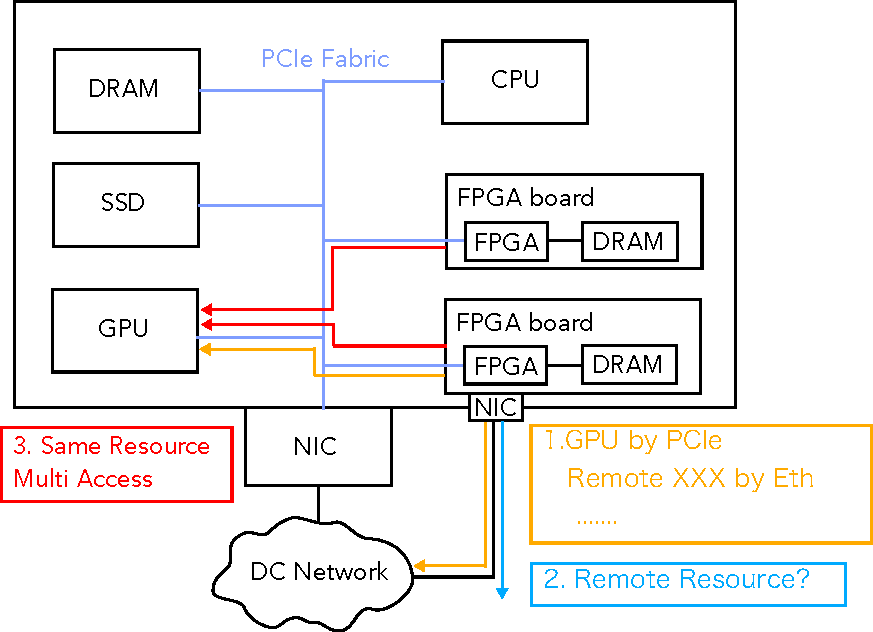
\includegraphics[scale=0.5]{fig/ez_FPGA_Base.pdf}
  \end{figure}
\pnote{
}
\end{frame}

% ============================ 各背景に対する問題提起と理想的なアーキテクチャ ===============================
\section{問題の解析と理想のアーキテクチャ(目的)}
\begin{frame}\frametitle{問題1}
	\begin{itemize}
		\item 異なるリソース/異なるリソースロケーション/異なる通信方式
			\begin{itemize}
				\item Resource: DRAM, CPU, GPU,  FPGA, ...
				\item Location: ローカルホスト、リモートホスト
				\item Stack: PCIe, network, ...
			\end{itemize}
		\item FPGAアプリケーションが何を利用するかによるが非常にプログラムが複雑になる。
		\item 表は各リソース、Stackの実装に何行程度必要かを示す図。
	\end{itemize}
  \begin{figure}[htb]
		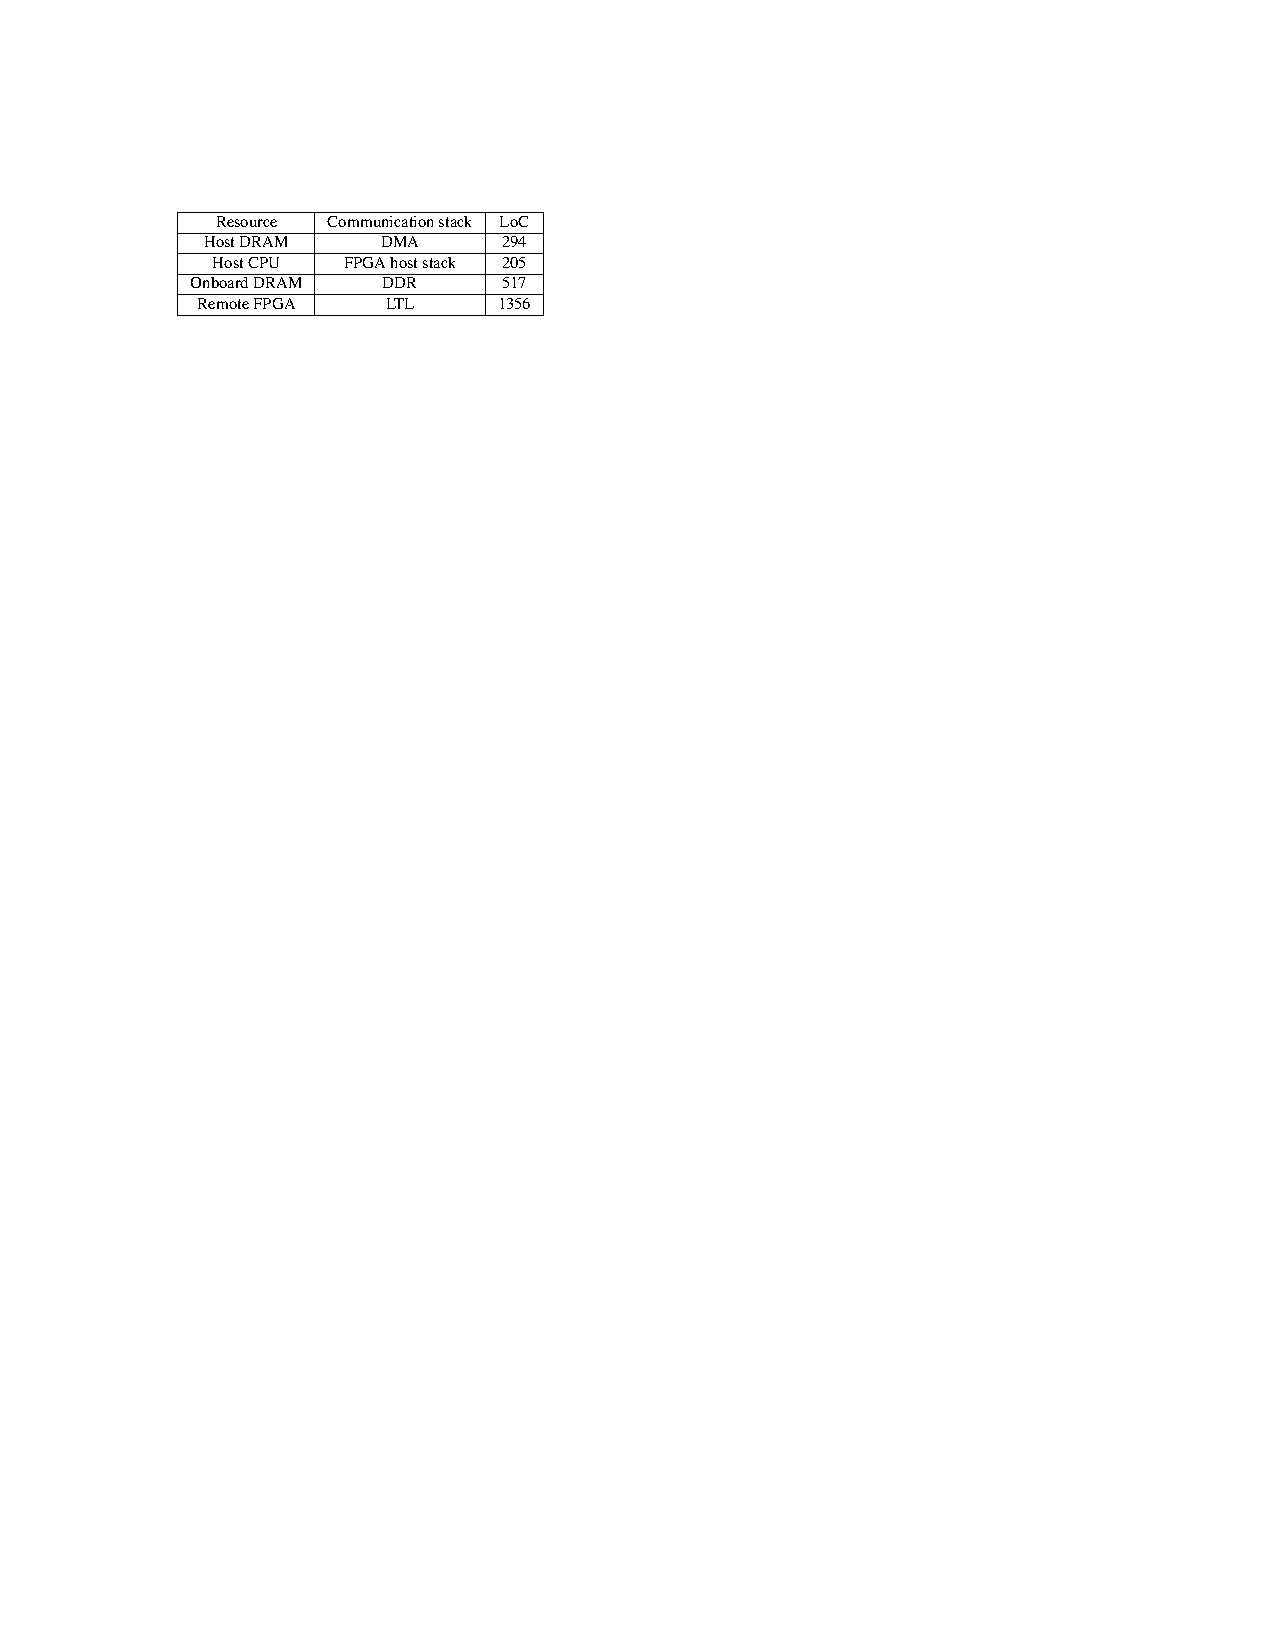
\includegraphics[scale=1.0]{fig/table1.pdf}
  \end{figure}
	\pnote{
	}
\end{frame}

\begin{frame}\frametitle{問題1へのアプローチ}
	\begin{itemize}
		\item common communication interface
		\item Applicationからは共通のインターフェースを利用するように抽象化
	\end{itemize}
  \begin{figure}[htb]
		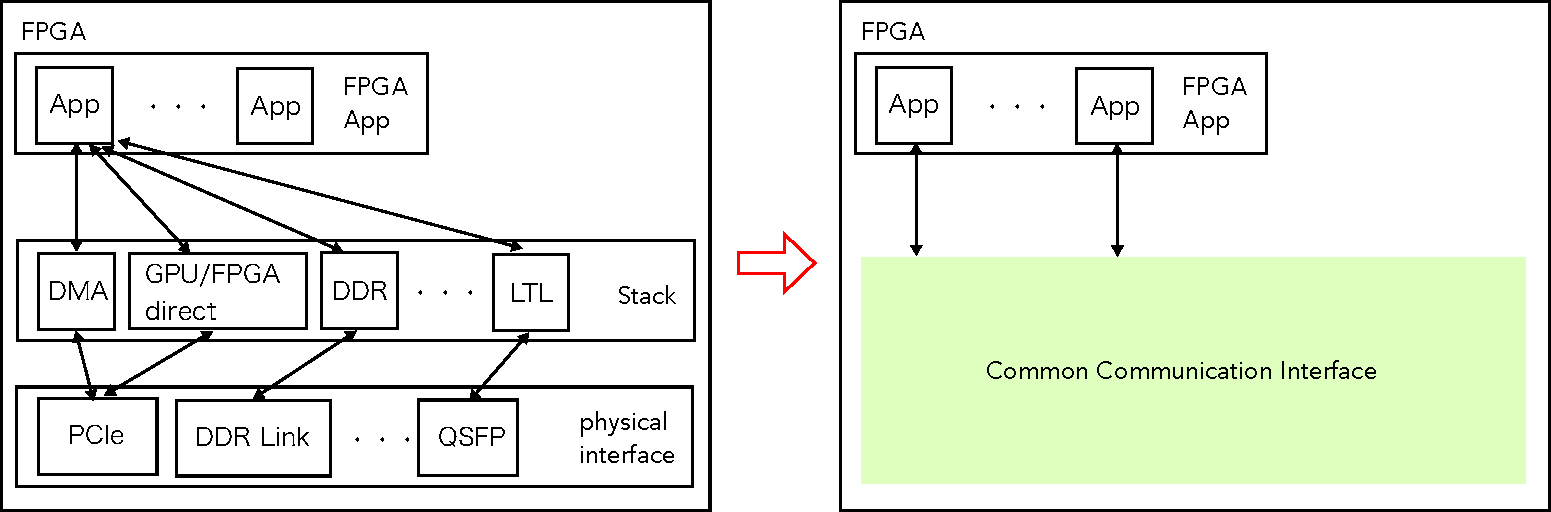
\includegraphics[width=\linewidth]{fig/ez_FPGA_common_communication_interface.pdf}
  \end{figure}
	\pnote{
	}
\end{frame}

\begin{frame}\frametitle{問題2}
	\begin{itemize}
		\item Server-Centric(Server中心のnamespaceによるアクセシビリティの悪さ)
			\begin{itemize}
				\item 例えばPCIeアドレスはそのホスト内部からの利用のみが可能なnamespace
				\item このままだとRemoteのPCIeを使えなくない?
				\item ローカルとリモートに別途daemon process建てるとか?
			\end{itemize}
			\item このような記述をリソースコミュニケーション種類ごとに記述する。
	\end{itemize}
	\pnote{
	}
\end{frame}

\begin{frame}\frametitle{問題2へのアプローチ}
	\begin{itemize}
		\item global unified naming scheme
		\item DCネットワークリソースを一意に特定するような命名をしてリソース特定可能にする。
	\end{itemize}
  \begin{figure}[htb]
		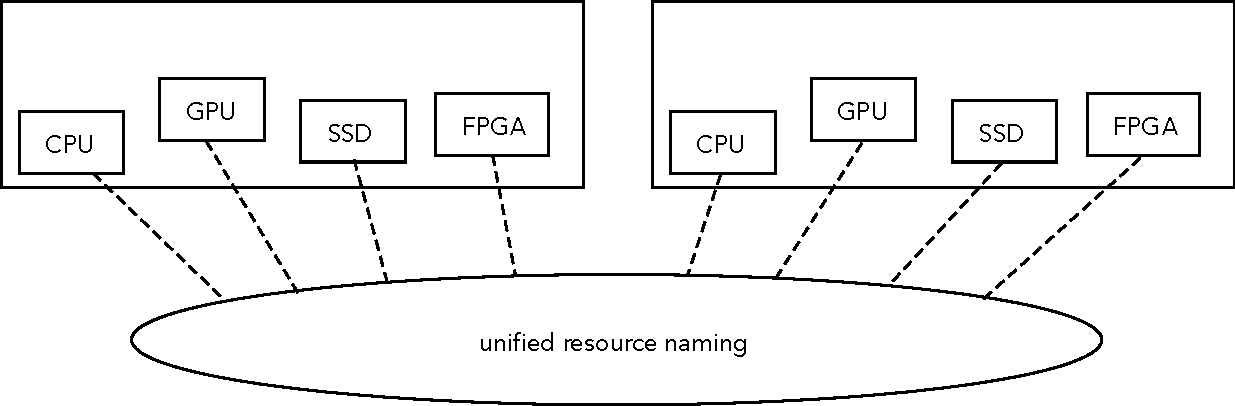
\includegraphics[width=\linewidth]{fig/ez_FPGA_unified_naming_scheme.pdf}
  \end{figure}
	\pnote{
	}
\end{frame}

\begin{frame}\frametitle{問題3}
	\begin{itemize}
		\item 通信におけるリソースマルチプレクシングが貧弱
			\begin{itemize}
				\item 例えばPCIeを利用するが、アクセス先はDMA/GPU/FPGAと異なる場合
				\item FPGA開発者はこれを適切にプログラムでハンドルする。
				\item Applicationと密結合になってしまう
			\end{itemize}
		\item 更に、同じリソースへの同時アクセスケースのハンドリングも。。。
			\begin{itemize}
				\item 2つのFPGA上のApplicationから同じSSDに書き込む場合
			\end{itemize}
	\end{itemize}
	\pnote{
	}
\end{frame}

\begin{frame}\frametitle{問題3へのアプローチ}
	\begin{itemize}
		\item underlying network serviceの実装
		\begin{itemize}
		  \item unified naming schemeを利用したリソースのRouting
			\item multiplexing機能も実装
		\end{itemize}
	\end{itemize}
  \begin{figure}[htb]
		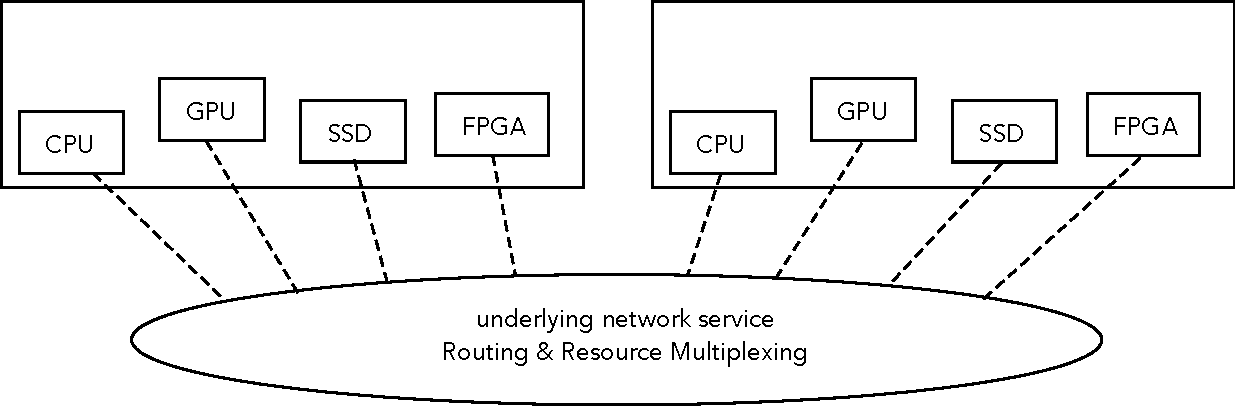
\includegraphics[width=\linewidth]{fig/ez_FPGA_mux_routing.pdf}
  \end{figure}
	\pnote{
	}
\end{frame}

\begin{frame}\frametitle{目的とDesicred Communication Architecture}
	\begin{itemize}
		\item まとめるとFPGAの世界に以下のようなアーキテクチャを導入したい
			\begin{itemize}
				\item common communication interface
				\item global, unified naming scheme
				\item underlying network service
			\end{itemize}
		\item これを実装したものが{\color{red} Direct Universal Access (DUA)}である。
	\end{itemize}
  \begin{figure}[htb]
		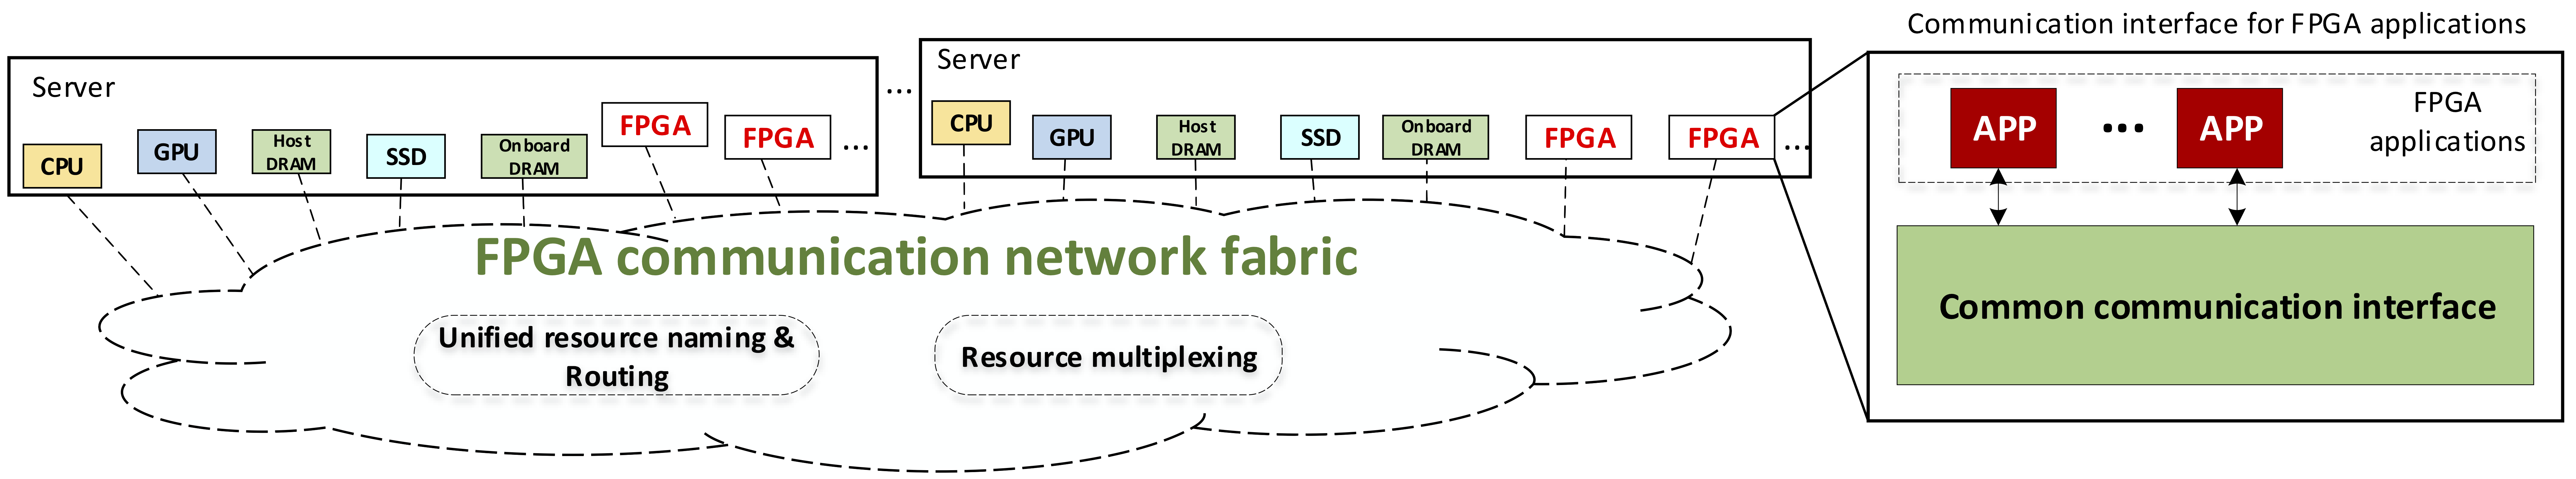
\includegraphics[width=\linewidth]{fig/figure1b.png}
  \end{figure}
	\pnote{
		以降ではglobal, unified naming schemeの話、common communication interfaceの話、underlying network serviceの話の順に話します。
		前者2つはサラッと行きますが、underlying network serviceが長いのでそのつもりで効いていただけるといいかと思います。
	}
\end{frame}

% =========================== DUA Components ===============================
\begin{frame}\frametitle{Resource Address Format}
	\begin{itemize}
		\item まずは{\color{red} global, unified naming scheme}の話から。
		\item DUAではDC内でグローバルにユニークなアドレスを各リソースにつける
		\item ただし新しいアドレスフォーマットを考えるのは懸命ではない $\rightarrow$ 様々なリソースの既存の命名法を活用する。
		\item UID = server ID : device ID : resource INST
			\begin{itemize}
				\item server ID : IP address
				\item device ID : 各サーバ内でuniqueなID
				\item resource INST: 各デバイスにおける既存のaddressing scheme
			\end{itemize}
	\end{itemize}
  \begin{figure}[htb]
		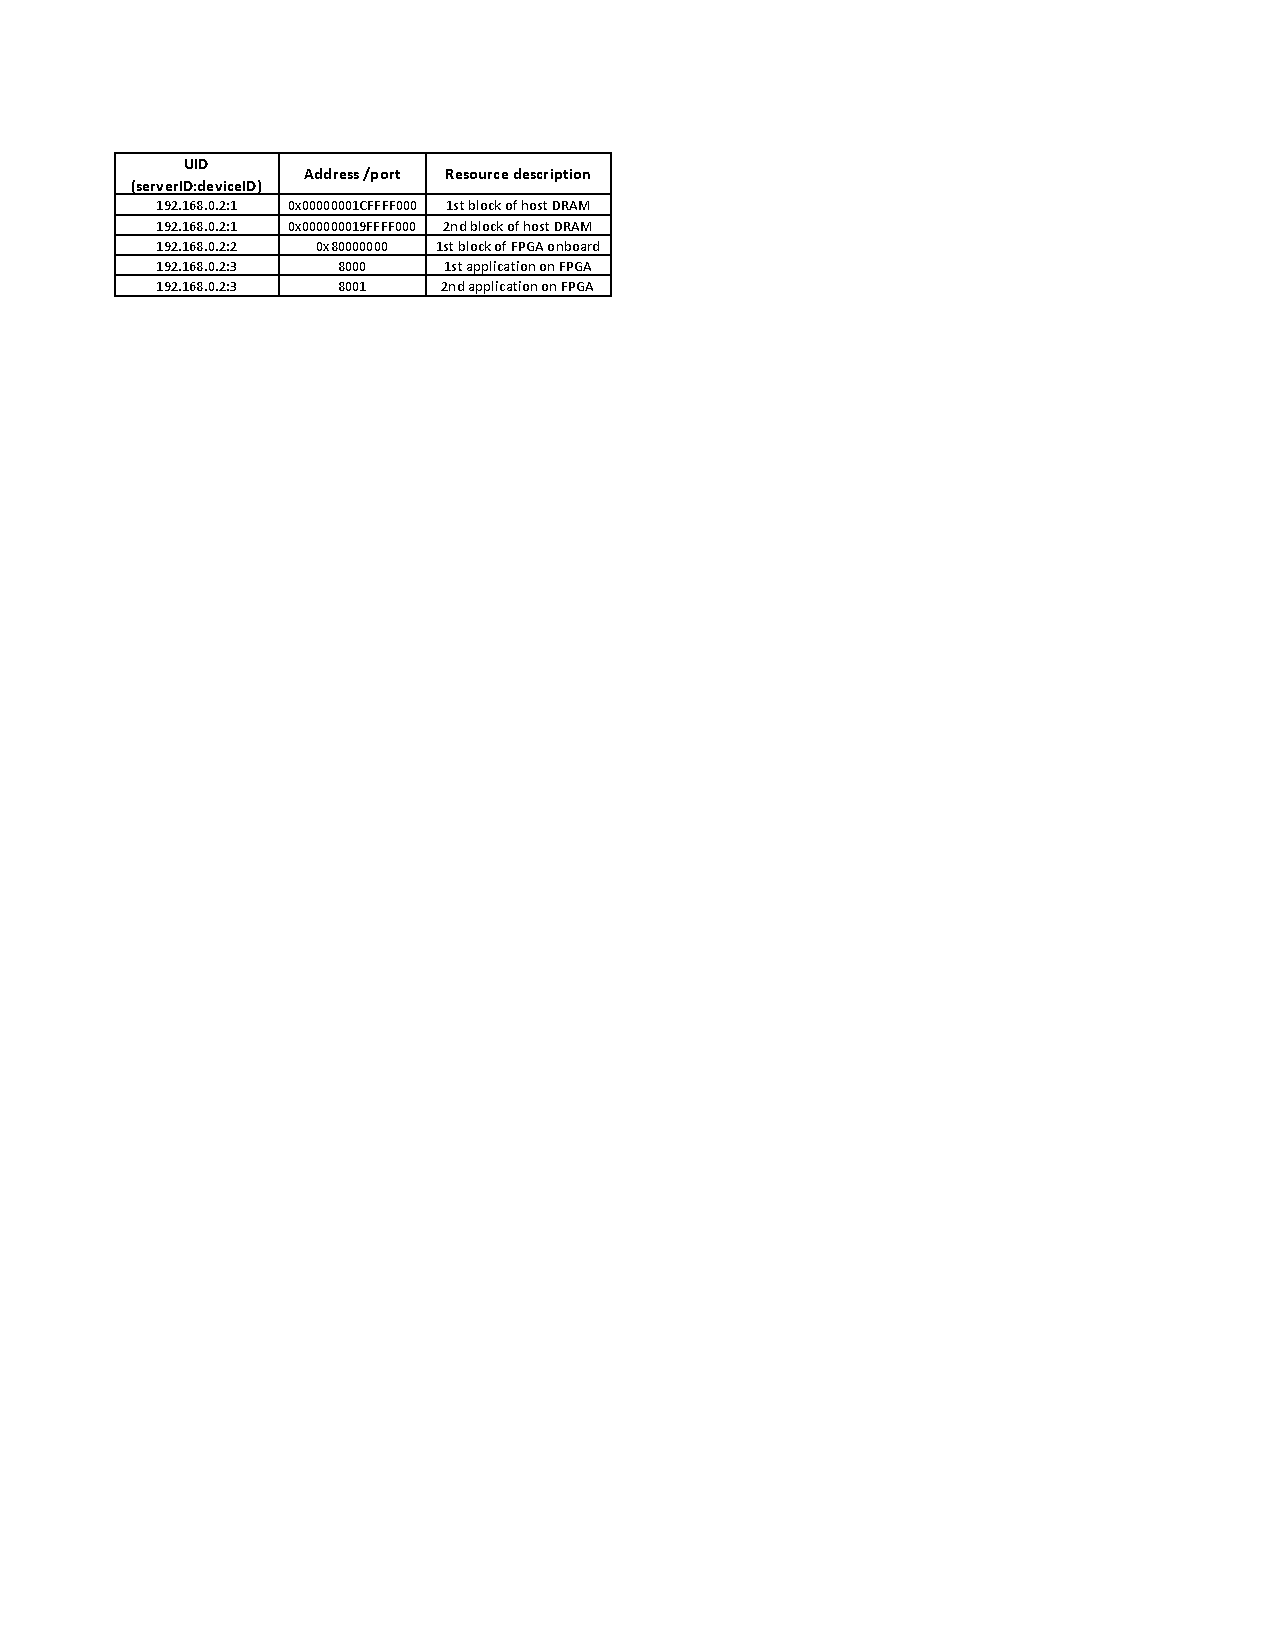
\includegraphics[scale=1.0]{fig/figure3.pdf}
  \end{figure}
\pnote{
	話の順番が列挙順と変わりますがまずは、global, unified naming schemeの話からします。
	というのも、これは共通インターフェースの話と、overlay networkの話両方に絡んでくるからです。
}
\end{frame}


\begin{frame}\frametitle{DUA Communication Interface}
	\begin{itemize}
		\item 次に、{\color{red}Common Communication Interface}の話
		\item 共通のインターフェース(API)
		\item プログラマはこのインターフェースを利用することのみを考えればいい。
			\begin{itemize}
					\item アプリケーションではBSDソケットのようなノリで取り扱える。
					\item Connection setup/close primitive (CONNECT/LISTEN/ACCEPT/CLOSE)
					\item Data transmittion primitive (SEND/RECV, READ/WRITE)
			\end{itemize}
		\item socketプログラミングみたいに両方で開いて送受信してクローズみたいな形のコード記述
	\end{itemize}
\pnote{
}
\end{frame}

\begin{frame}\frametitle{DUA underlay network}
	\begin{itemize}
		\item 最後に、{\color{red}Underlying network service}の話(これが長い。。。)
		\item 全体像の俯瞰図が下図
		\item 大きく分けてControl Plane / Data Planeに分かれている
		\item これらの協調作業によりRoutingやResource Multiplexing を実現する
	\end{itemize}
  \begin{figure}[htb]
		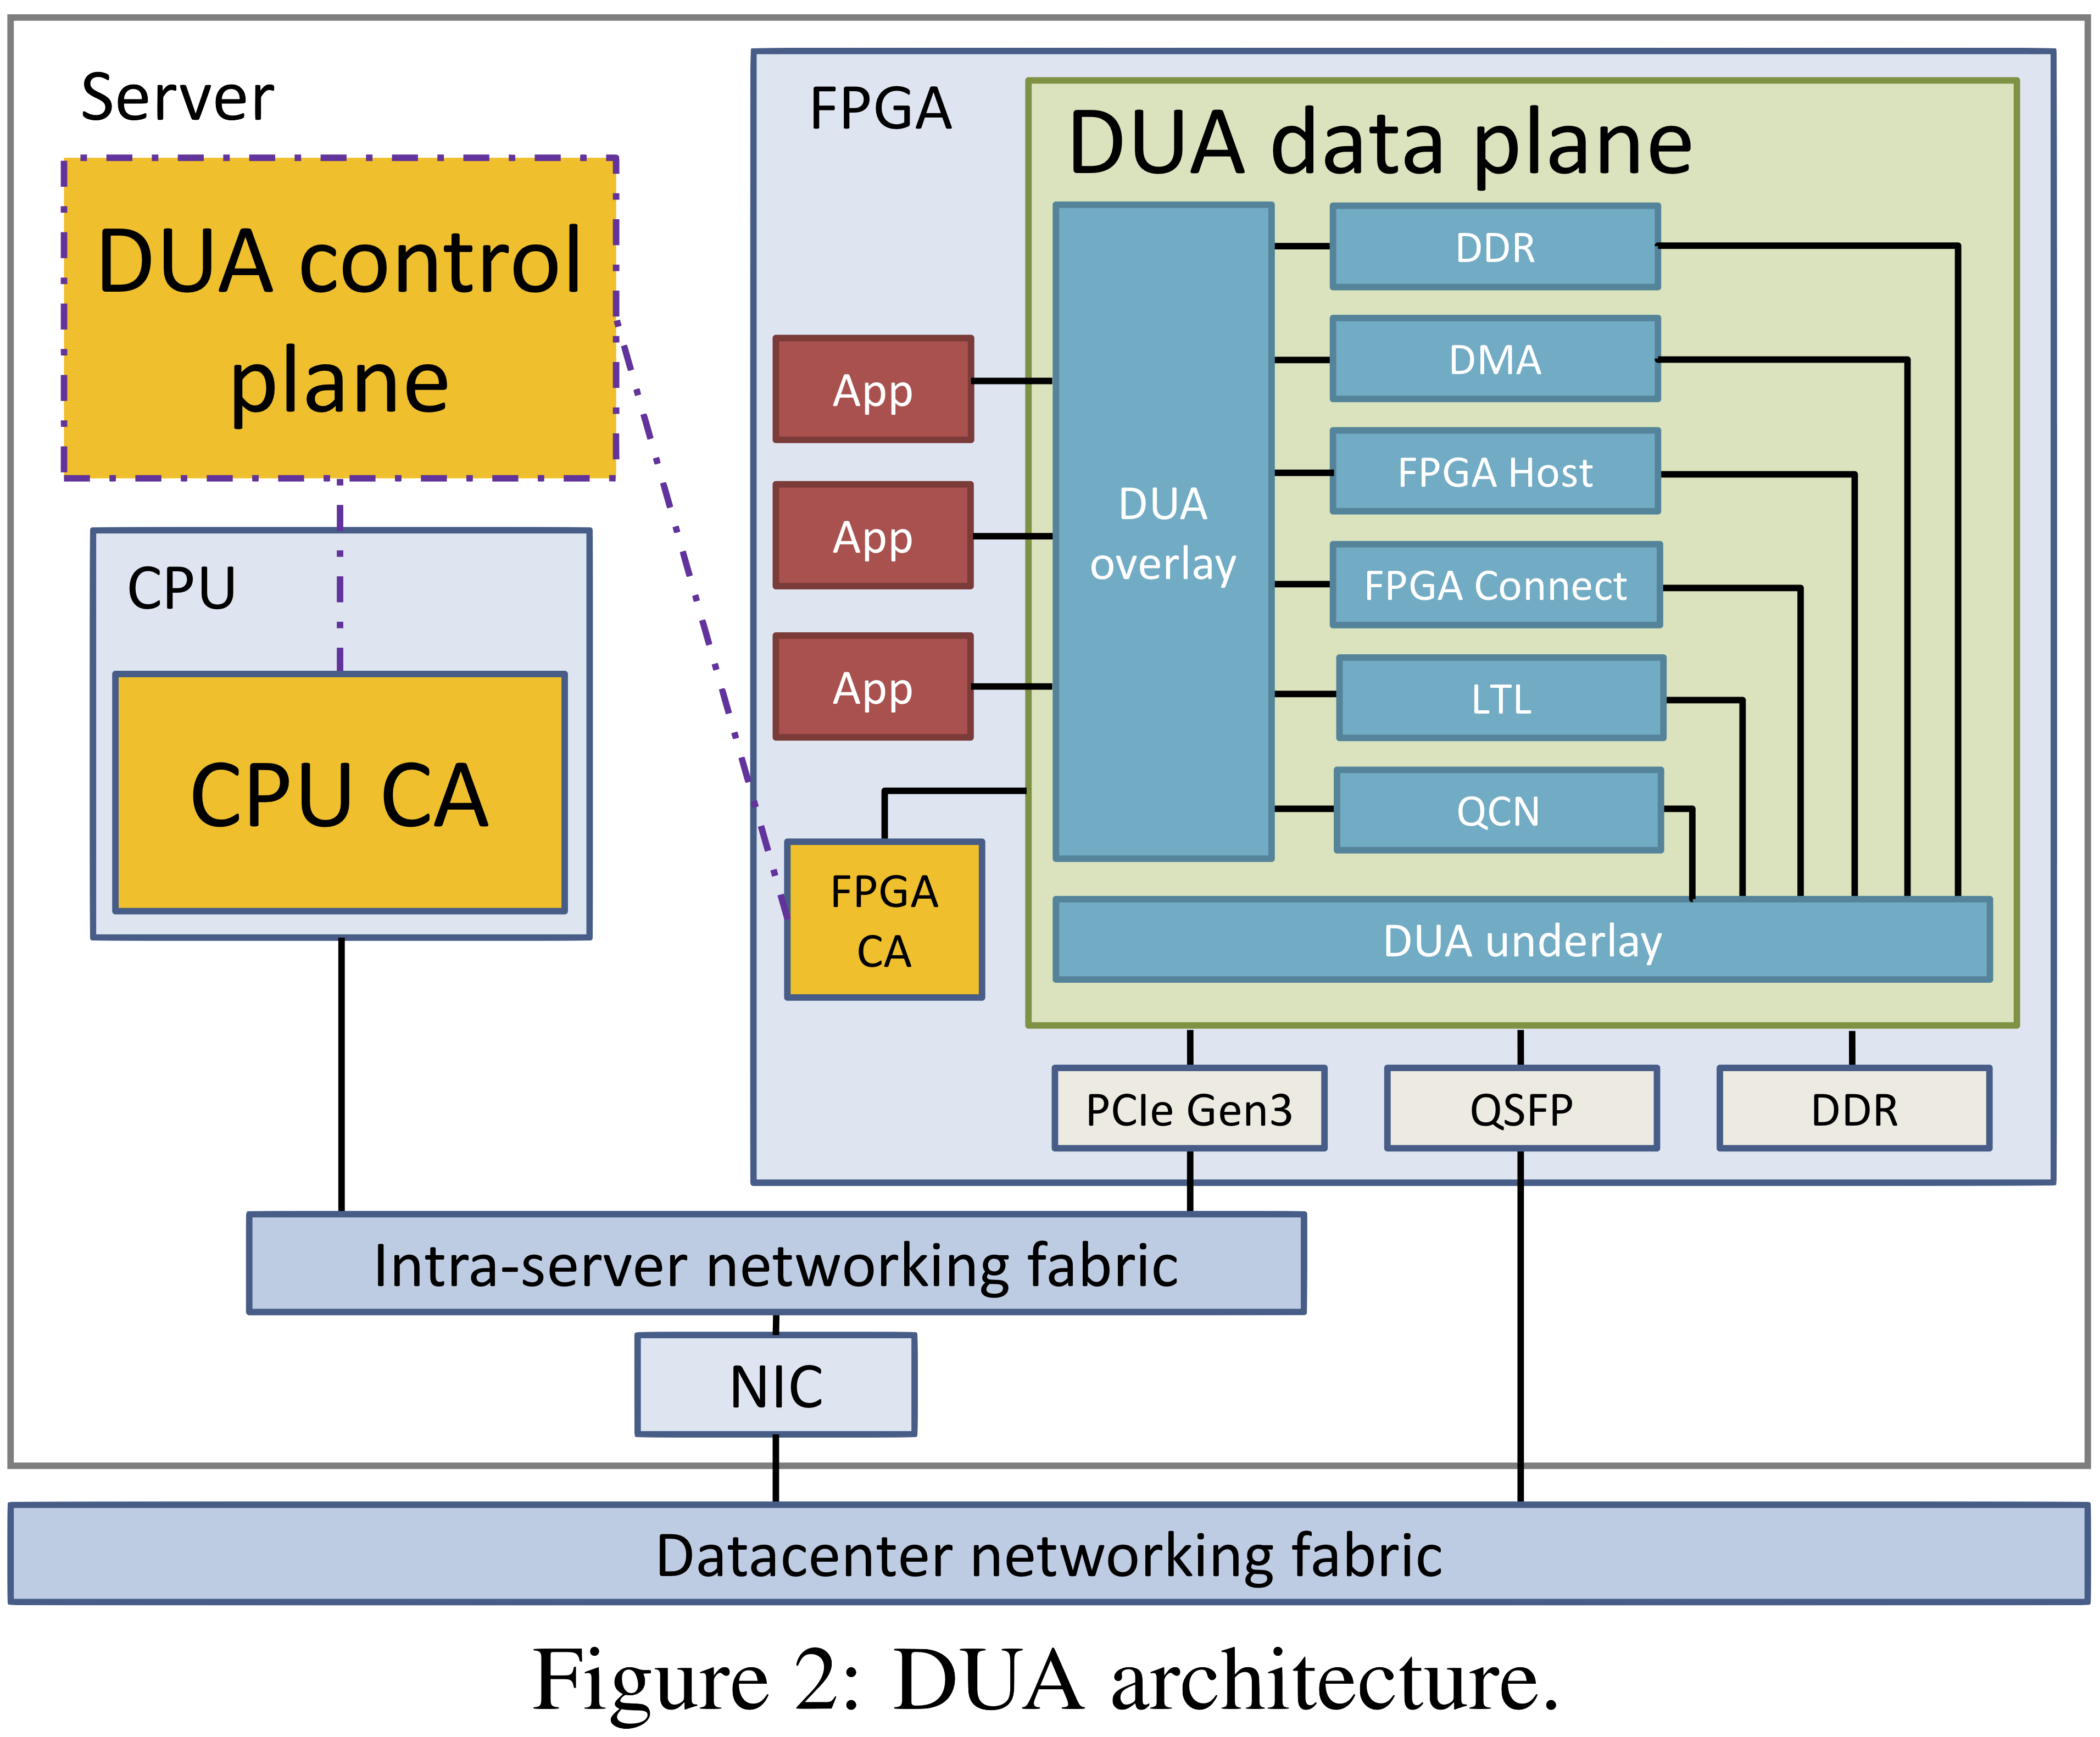
\includegraphics[scale=0.6]{fig/figure2.png}
  \end{figure}
\pnote{
}
\end{frame}


% 各通信インターフェースのStackはそのまま利用し、これはあくまでDUAの話というとをごっちゃにしないように伝える
\begin{frame}\frametitle{DUA Control Plane}
	\begin{itemize}
		\item まずDUAのControl Plane
		\item CPU Control Agent (CPU CA)とFPGA Control Agent (FPGA CA)
		\item CPU / FPGA CAで{\color{red} Resource Management, Routing Management, Connection Management}を行う
	\end{itemize}
  \begin{figure}[htb]
		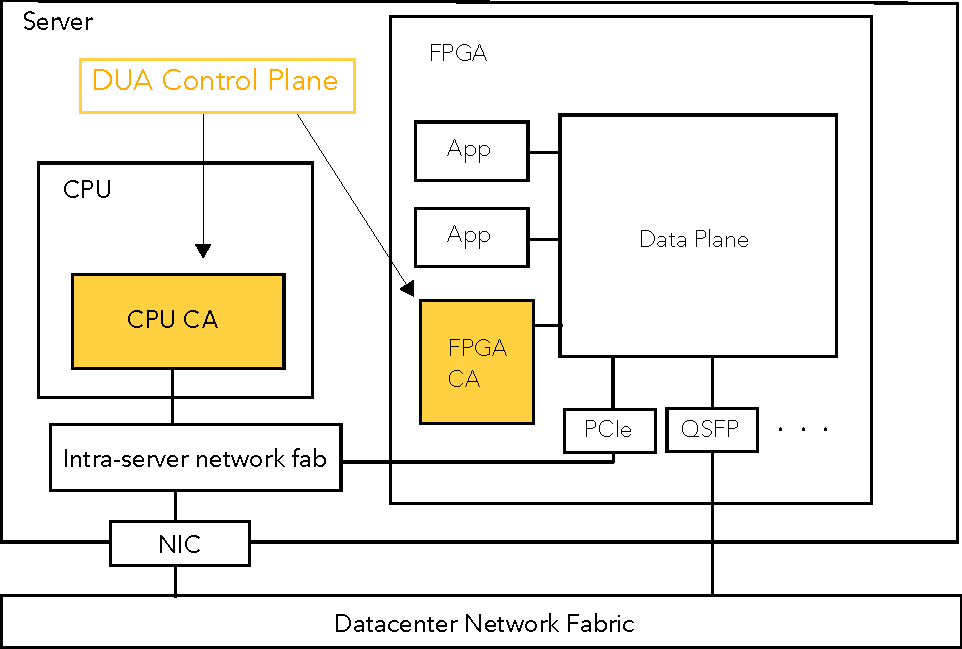
\includegraphics[scale=0.4]{fig/ez_DUA_ControlPlane.pdf}
  \end{figure}
\pnote{
	次のスライドから, ResourceManagement, Routing Management, Connection Managementを順に見ていきます
}
\end{frame}

% cpu caで管理しているのはdevice idのみ?
% ip addressはまぁ共通だし。
% リソース内のアドレスは管理せずデバイスに制御させると書いてある。
\begin{frame}\frametitle{Resource Management}
	\begin{itemize}
		\item FPGA CAがオンボードのリソースに関する情報をCPU CAに伝える
		\item CPU CAは上記 + その他メモリ/GPU情報などを集めUIDを割り当てる
			\begin{itemize}
				\item device IDはホストでユニークに降るため、CPU CAはdevice IDとローカルリソースのmappingを持っている。
				\item もちろんplug-in/plug-out/failureなどでリソース変更が起きた際にはmappingのupdateを行う。
			\end{itemize}
		\item 現実装ではまだnaming serviceはないためUID指定でリソース利用する
	\end{itemize}
  \begin{figure}[htb]
		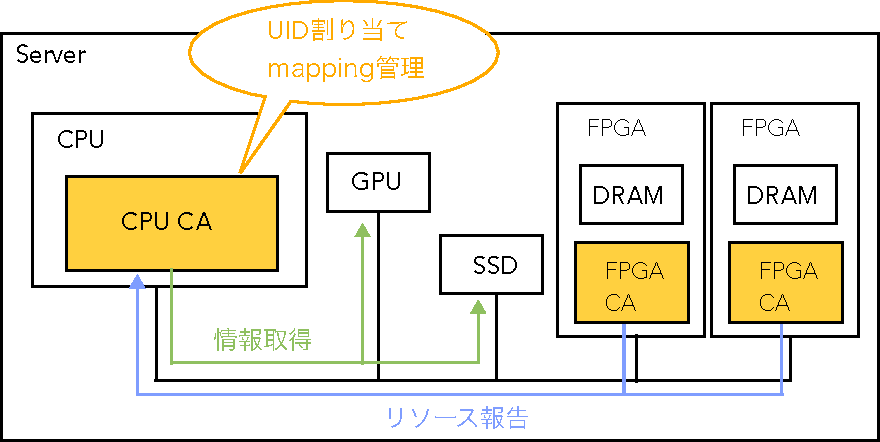
\includegraphics[scale=0.4]{fig/ez_DUA_ControlPlane_ResourceMangement.pdf}
  \end{figure}
\pnote{
}
\end{frame}

\begin{frame}\frametitle{Routing Management}
	\begin{itemize}
		\item 各サーバー内のリソースの接続情報からrouting pathを決定する。
		\item FPGA CAがcommunication stack と physical interfaceの情報をCPU CAに伝える
		\item CPU CAは各サーバーごとにinterconnection tableを保持、管理しこれをもとにrouting pathを決める
			\begin{itemize}
				\item ただしDC network fabricとの接続性を確認した場合は、他サーバのあるリソースを意味するエントリーを挿入する。
			\end{itemize}
		\item FPGA1(192.168.0.2:4) $\rightarrow$ FPGA3(192.168.11.5:3/On Remote Host)のルーティングパスは、\\ {\color{orange} FPGA1 $\rightarrow$ (FPGA Connect) $\rightarrow$ FPGA2 $\rightarrow$ (LTL) $\rightarrow$ FPGA3}
	\end{itemize}
  \begin{figure}[htb]
		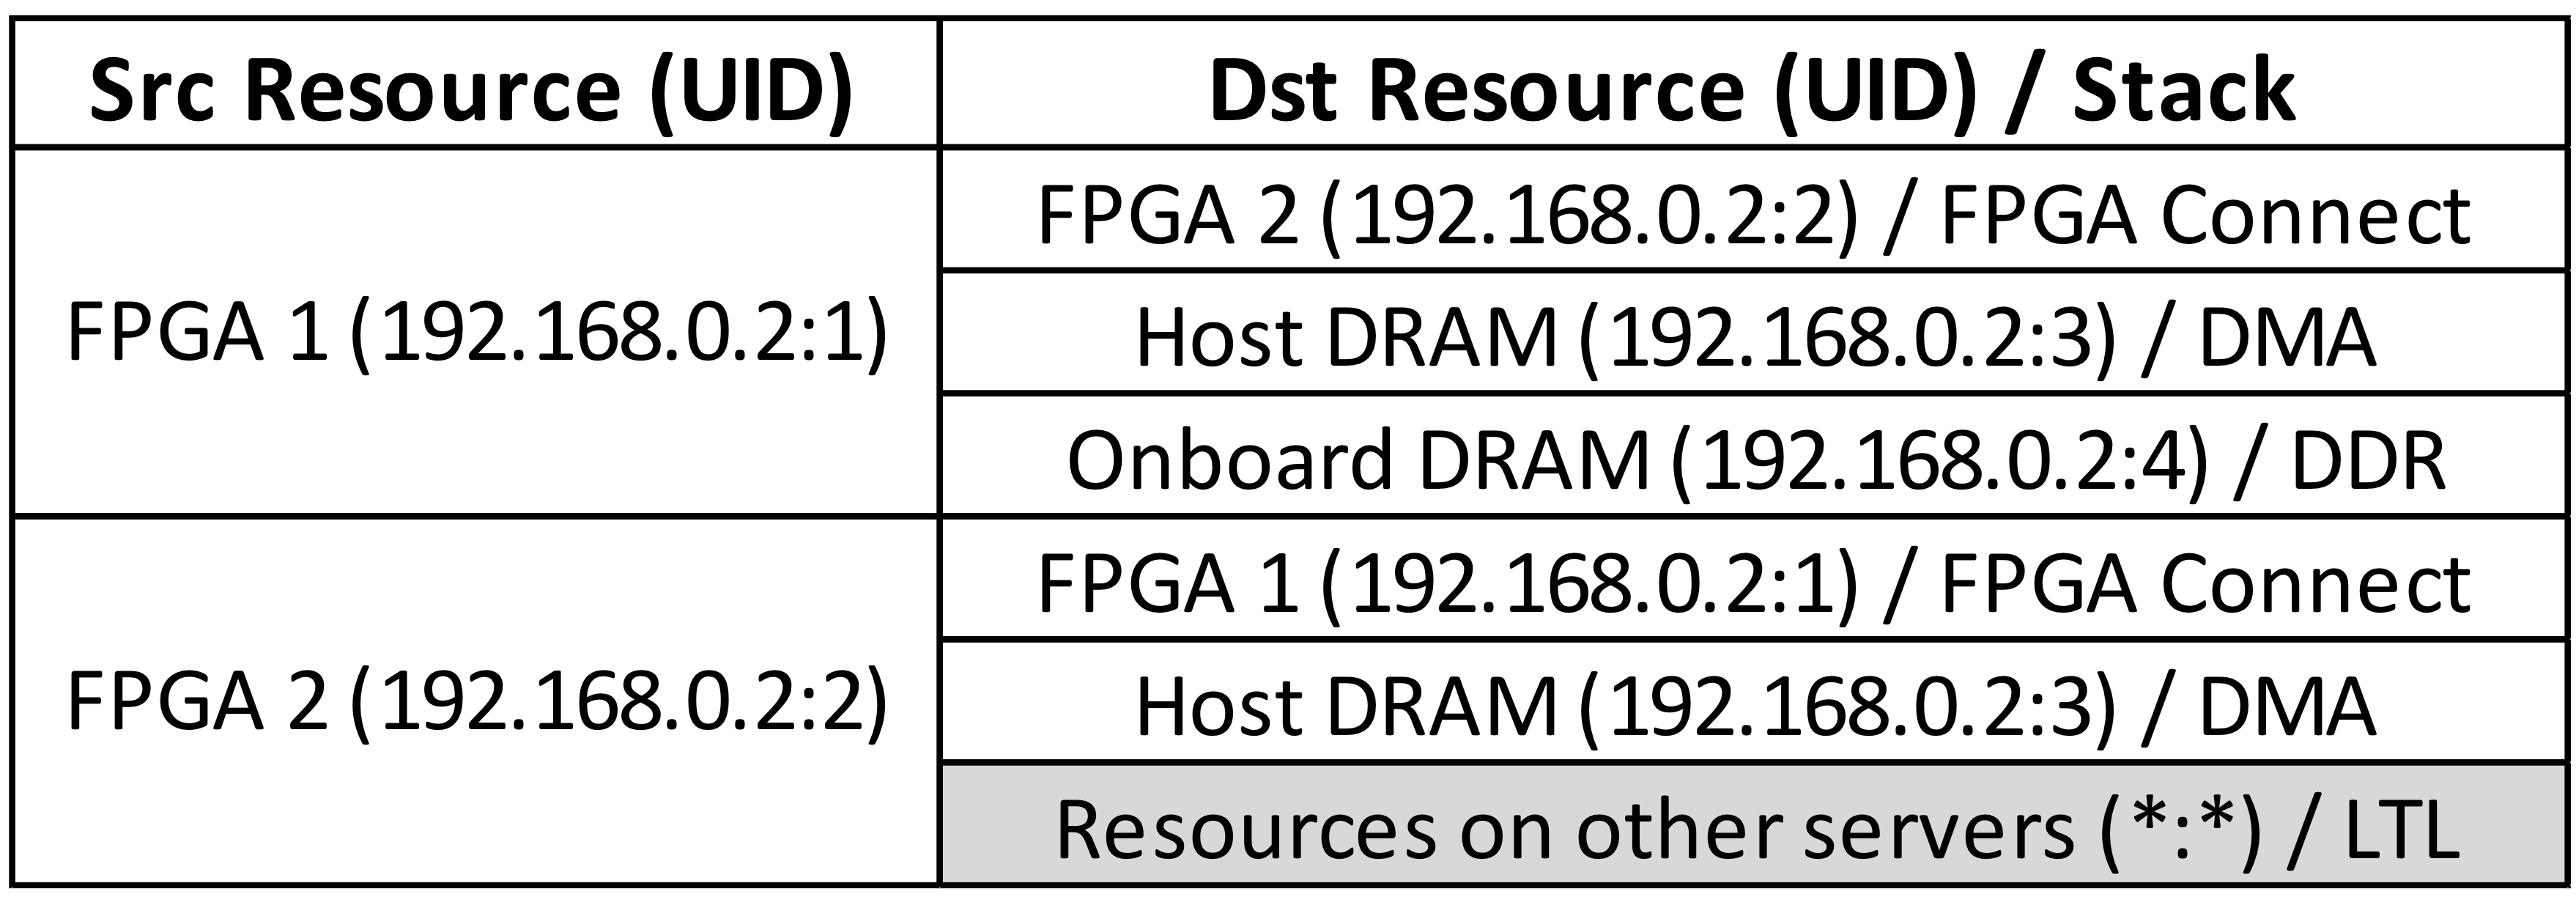
\includegraphics[scale=1.0]{fig/figure5.png}
  \end{figure}
\pnote{
	innterconnection table : スライドの表にあるやつ
	あるソースリソースに対して、他の各リソースにどのように接続できるかをまとめた表
	interconnectionの情報自体の収集はFPGA CAからの通知などから取得する
	これを元にRouting Pathを決める

	以下、メモ

  ここでいうroutingとは。。。?
  もちろんDC Networkでのroutingではない。これは今回の例でいうとLTL(UDP/IP上に定義されるプロトコルでFPGA間の通信に利用されるもの)
  routingとは各サーバー内の接続情報から、各サーバー内部のrouting pathを決定する部分。つまりDUA overlayの部分のルーティングという意味になりそう
  CPU CAは各サーバーのinterconnection tableを保持する。全てのローカルリソースに関するinterconnect情報で、UIDを利用する? (正確にはCPU CAはdeviceIDを保持しているのでUIDがわかっている、という感じか)。
  第一カラム : src FPGA
  第二カラム : dst resource (can accessed from this FPGA through which underlying communication stack)
  つまり1 : Nの構成テーブル
  
  table upload
  1. FPGA CAがcommunication stack と physical interfaceの情報を自サーバーのCPU CAにuploadする。
  2. CPU CAは(同一ホストの)異なるFPGA間のinterconnectonを決定し、interconnection tableを更新する。↑
  3. あるFPGAがDC network fabricとの接続性を報告したとき、他サーバのあるリソースの情報の意味を持つエントリーを挿入する(これはいまいちspecificでないがこれだけの情報があればいいのか?)
  
  このinterconnection tableでターゲットリソースへのrouting pathが用意に計算できる。 (packetは後で出てくる)
  1. destination UIDから、serverID, deviceIDを確認し、同一FPGAからdirect connectionできるかどうかを確認し、interconnection tableにあるstackを利用してリソースアクセスする。
  2. そうでない場合、interconnection tableから他のFPGAを介すようなrouting pathを見つける。
  
  ex.  Figure5にて。
  FPGA1 (192.168.0.2:4) が他のサーバーに位置しているFPGA3(192.168.11...5:3)のapplicationに通信したいいとき、ルーティングパスとしては以下が計算される。
  FPGA1 -(FPGA Connect)-> FPGA2 -(LTL)-> FPGA3
  
  lookupの方針によっては本来望ましい最適なpathを通らない可能性がある気はする。到達はしそうだが。
  -> いや言い方が悪いな、もしlookup時にstep1が早い想定だと、latencyが上る可能性がある、くらいの温度感か。なのでlookup速度の差くらいはありそう程度
}
\end{frame}


\begin{frame}\frametitle{Connection Management}
	\begin{itemize}
		\item Connectionの管理もControl Planeで行う。
		\item まずアクセス可能かどうかをpolicyで判断し、良ければrouting pathを決定してそれに沿ったforwarding tableをデータプレーンに配る
		\item Stackによっては大量同時接続が非サポートのこともある(LTLは64しかない)が、複数のDUA connectionを同一のtunnel connectionでマルチプレクシングできる
		\item ApplicationがコネクションをクローズしたときにはStackのtunnel connectionをクローズしforwarding tableをdata planeから削除する。
		\item コネクション成立/失敗時にアプリケーションに通知する
	\end{itemize}
\pnote{
	以下、メモ

  DUAでは各FPGA communicationはconnectionとして抽象化され、<srcUID:dstUID>のペアで識別され、これもControl Planeで管理される。
  step1. Connection phase
    1. アクセスコントロールポリシーを確認する。src FPGA applicationがdst resourceにアクセス可能かの確認をする。
    2. OKならdestへのrouting pathを計算し、routing pathに沿ったフォワーディングテーブルをFPGA data planeに配る。
    3. data planeはこれに従ってforwardingするため、適切なcommunication stackを利用することができる。
    4. routing pathの種類によって CPU CAは異なるアクション(?<- 多分これVirtual Networkの意味での用語のactionで使っている気がする)をデータプレーンとunderlying stackに流すことができる
 			1. dst resourceがdirect connected -> CPU CAは単純に対応するforwarding tableをデータプレーンに流す。
 			2. dst resourceがdirect connectedではないが同一サーバー -> CPU CAはルーティングパスに沿ってローカルFPGAのstackを呼び出しconnectionをsetupする。
         冷静に考えてこのFPGA間のconnectionもないので実装したのでは?という気持ちがある。
         ex.
         Figure5にて、FPGA2がFPGA1のオンボードDRAMにアクセスするために接続開始したとき、CPU CAはFPGA2とFPGA1の間にFPGA Connect connectionをsetupする。
 			3. dst resourceがリモートサーバのリソース -> CPU CAはリモートのCPU CAと強調してFPGA間のconnection tunnelをLTLなどでセットアップする
 
  step2. established phase
 		1. step1が全てうまく行くと、DUA connection establishedになる。
    2. establishedになるとapplicationにその旨の通知が飛ぶ。
    3. いくつかのstackでは多くの同時接続がサポートされていなかったりする(LTLは64しかない)が、同一のrouting pathを持つ複数のDUA connectionは同一のtunnel connectionで多重化できる
       それ以外にも、各traffic classで複数のtunnelを用意しtraffic schedulingを容易にしたりもできる。
 
  step3. connecton close phase
 		1. applicationがconnectionをcloseするとき、DUAはstack tunnel connectionをクローズする(もちろん多重化されてなければ)
 		2. 対応するフォワーディングテーブルをdata planeから削除する。
    3. もしデータパス(targeted resource, physical interface, comunication stack)で何かしらの失敗が発生したら影響のあるDUA connectionを削除しapplicationに通知する。
}
\end{frame}


\begin{frame}\frametitle{DUA Data Plane}
	\begin{itemize}
		\item 次にDUAのData Plane
		\item overlay, stack, underlayからなる。
			\begin{itemize}
				\item overlay  : 異なるApplicationとStackの間のデータ転送を行うRouter
				\item stack    : 既存のcommunication stack
				\item underlay : stack と physical interfaceをつなぎ、異なるstack用に物理インターフェース上でmultiplexingする
			\end{itemize}
	\end{itemize}
  \begin{figure}[htb]
		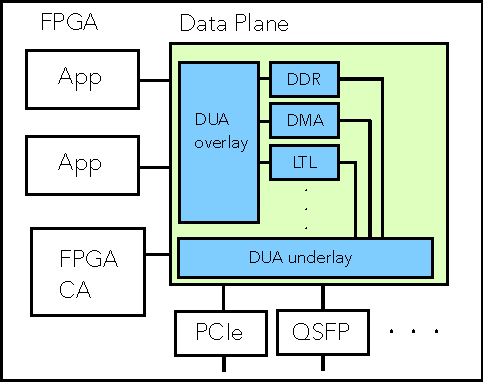
\includegraphics[scale=0.5]{fig/ez_DUA_DataPlane.pdf}
  \end{figure}
\pnote{
}
\end{frame}


\begin{frame}\frametitle{DUA Overlay}
	\begin{itemize}
		\item overlay部は更に、Connector, Switch Fabric, Stack Translatorに分かれる。
	\end{itemize}
  \begin{figure}[htb]
		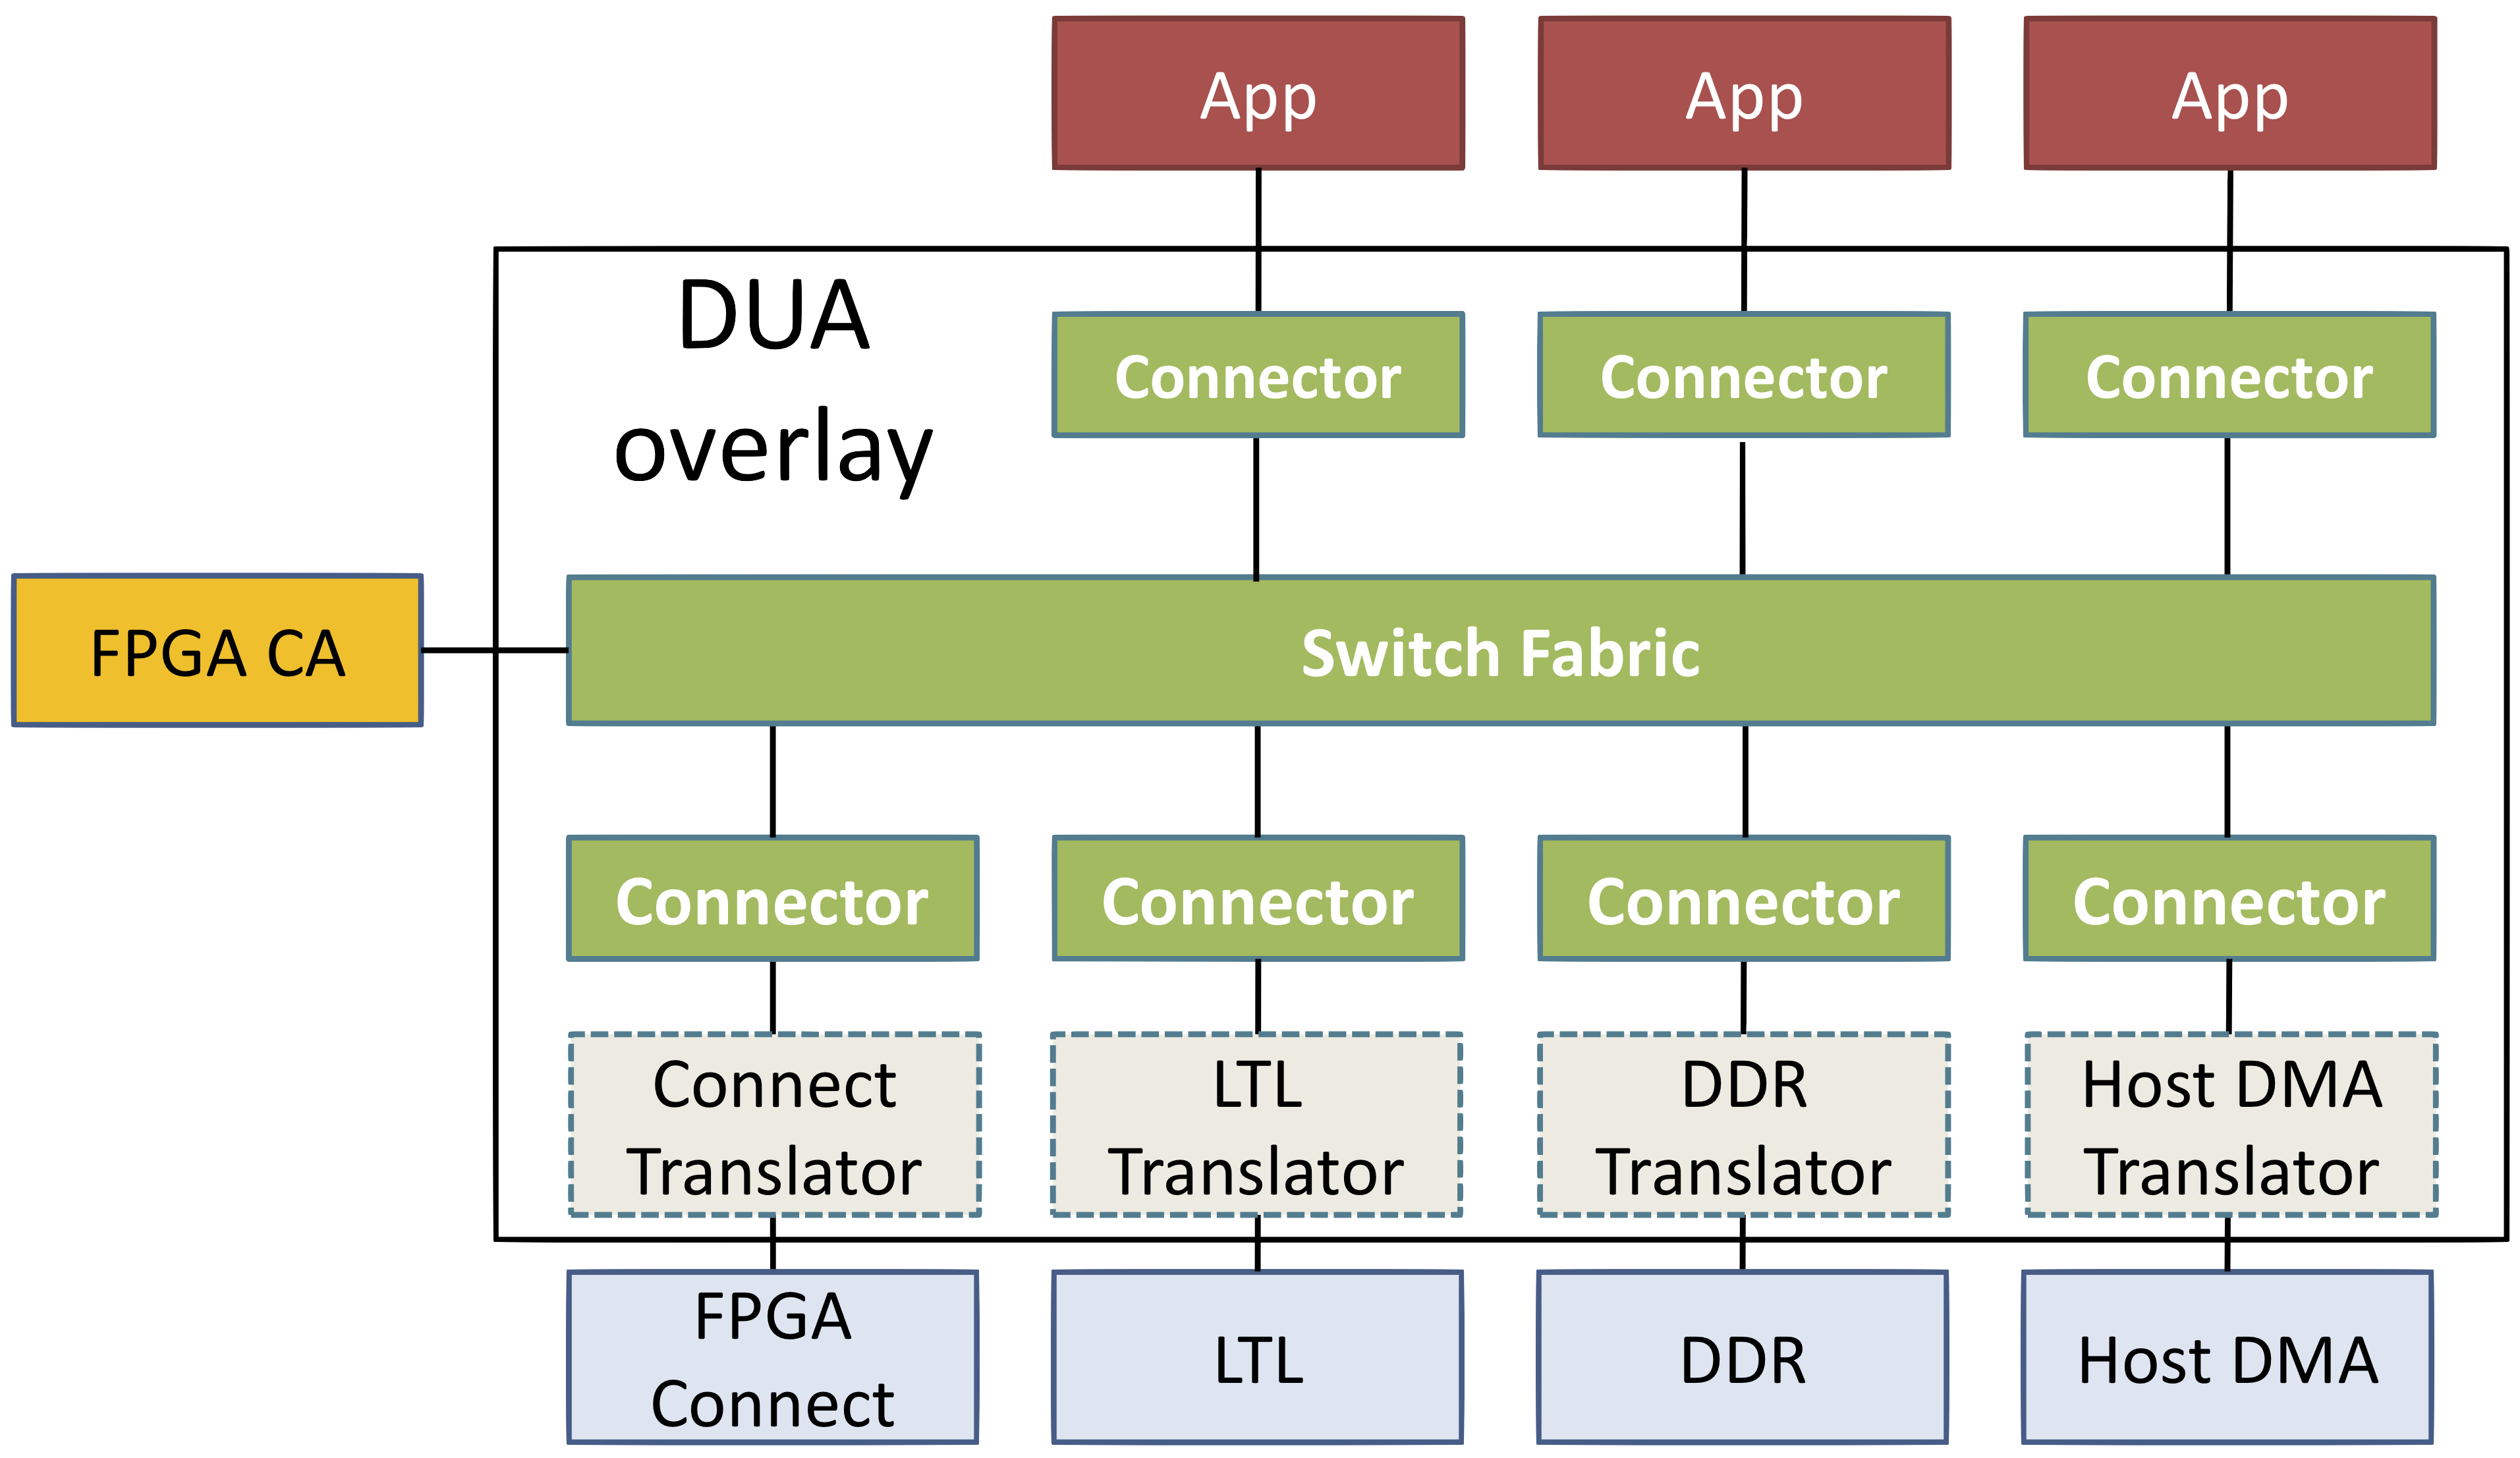
\includegraphics[scale=1.0]{fig/figure6.png}
  \end{figure}
\pnote{
	次はこれを順番に説明していきます
}
\end{frame}

% うまく短い言葉でまとまらないな。。。
% connectorはforwarding tableを持っている
% forwarding tableはUIDとswitch fabric の output portのmapping情報
%
% connector
% 1. encapsle data to DUA message
% 2. forwarding tableをlookupして、switch fabricを通してdestination connectorにmessageを転送するためにswitchのoutput portを決定する。
% 3. forwarding tableはControl PlaneからDUA Connectorへと配信される。
\begin{frame}\frametitle{DUA Overlay - Connector}
	\begin{itemize}
		\item App/Stack と Switch fabricの間に存在する。
		\item 主に2つの機能がある。
			\begin{itemize}
				\item データ転送 : I/O interfaceからのデータをencapし(DUA message)switch fabricへ転送する / switch fabricからのDUA messageをdecapし後続へ。場合によってはFPGA CAへ。
				\item forwarding tableの管理とlookup : forwarding tableに沿って転送先portを決定する
				\item Access control : CPU CAでpolicyに基づいたrouting path / forwarding tableが決まり、policy準拠のpathのみが許される。
			\end{itemize}
	\end{itemize}
\pnote{
	次の図を見せながら説明するといい
}
\end{frame}


\begin{frame}\frametitle{DUA Overlay - Connector}
	\begin{itemize}
		\item Connectorを図にするとこんな感じ
		\end{itemize}
  \begin{figure}[htb]
		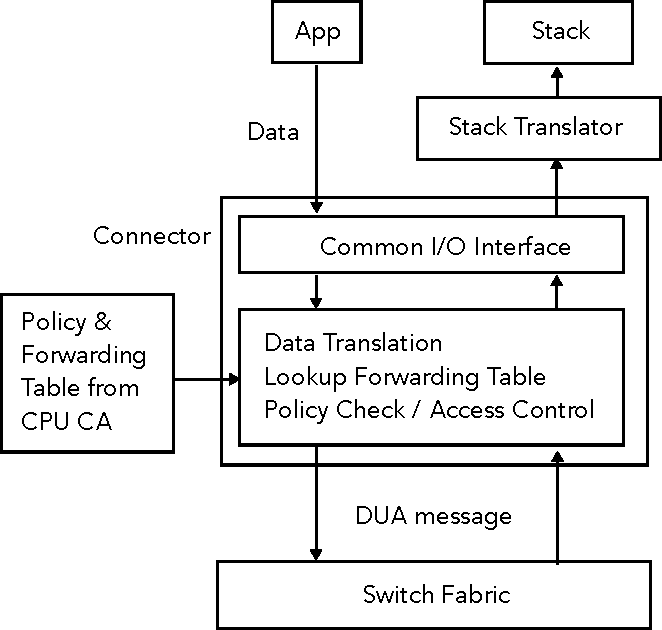
\includegraphics[scale=0.5]{fig/ez_DUA_DataPlane_Connector.pdf}
  \end{figure}
\pnote{
}
\end{frame}


% losslessにし、というがどういうことや
% application data buffer / stack data bufferって?
\begin{frame}\frametitle{DUA Overlay - Switch Fabric}
	\begin{itemize}
		\item App/Stack connector間に存在する
		\item incoming connectorからdestination connectorへmesageをswitchする
		\item バッファの話など細かい話があったがイマイチ何が言いたいのかわからなかったのと細かい話なので飛ばします。。。
	\end{itemize}
\pnote{
}
\end{frame}

\begin{frame}\frametitle{DUA Overlay - Stack Translator}
	\begin{itemize}
		\item Stack側ConnectorとStackの間に存在する
		\item DUA interfaceを実際のStackのinterfaceへ変換する
		\item Control Planeがconnection設立時にstack translatorに対応するtranslation tableを各stack translatorへ送る
		\item translation tableは、DUA message headerとunderlying stack headerのmapping情報でこれを元に変換する
		\item multiplex stack tunnelもここで制御できるらしい
	\end{itemize}
\pnote{
	次の図を見せながら説明するといい
}
\end{frame}

\begin{frame}\frametitle{DUA Overlay - Stack Translator}
	\begin{itemize}
		\item Stack Translatorを図にするとこんな感じ
		\end{itemize}
  \begin{figure}[htb]
		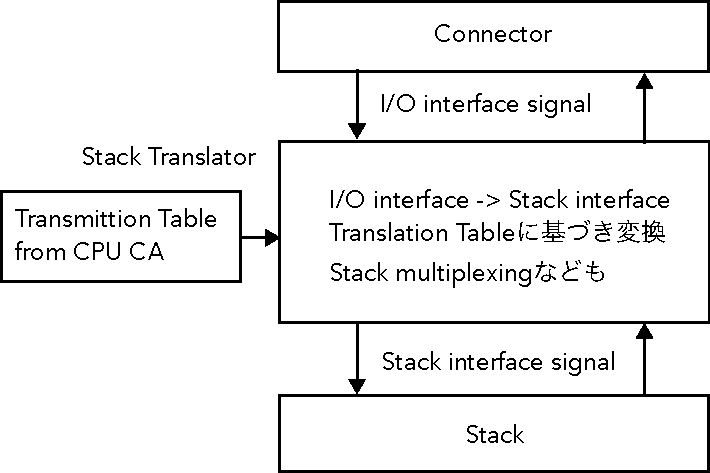
\includegraphics[scale=0.5]{fig/ez_DUA_DataPlane_StackTranslator.pdf}
  \end{figure}
\pnote{
}
\end{frame}


\begin{frame}\frametitle{Communicaton Stack}
	\begin{itemize}
		\item 現実装では、既存の4つのStack(LTL,DMA,FPGA-Host,DDR)をData Planeに統合した。
		\item DUAはend-to-endのtransport protocolにLTLを採用している。
			\begin{itemize}
				\item LTL (Lightweight Transport Layer)
				\item FPGA間のネットワークを介した通信でUDP/IP上に定義されるプロトコルらしい。
				\item DCネットワークの通信をFPGAから行うために利用し、輻輳制御はdisableらしい。
			\end{itemize}
		\item ただ、独自実装したFPGA Connect というStack (こちらはPCIe接続しているFPGA間での通信)も利用している
	\end{itemize}
\pnote{
}
\end{frame}

\begin{frame}\frametitle{FPGA Connect Stack}
	\begin{itemize}
		\item 単一サーバー上にPCIeで接続された異なるFPGA間で動作する複数Application間のdirect communicatonをサポートする
		\item スライドでは詳細は省略。
		\item Microsoft氏はこれもDUAのData Planeに組み込んでいるよう。
	\end{itemize}
  \begin{figure}[htb]
		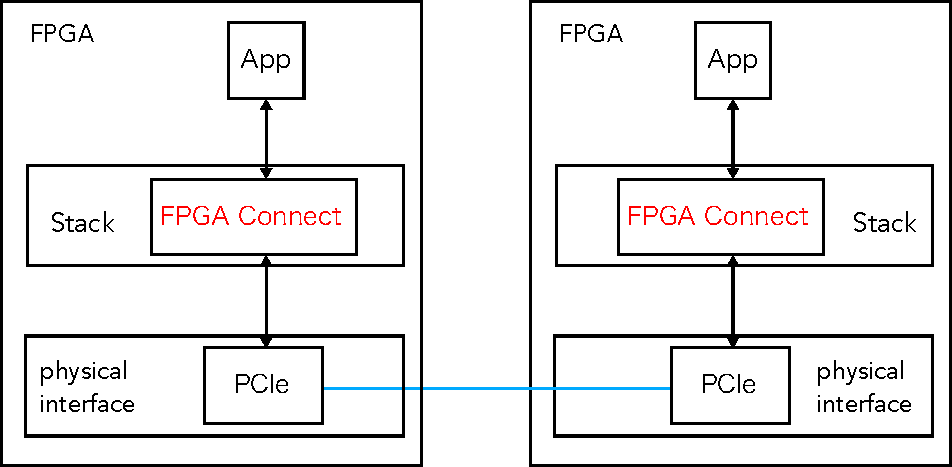
\includegraphics[scale=0.5]{fig/ez_FPGA_Connect.pdf}
  \end{figure}
\pnote{
}
\end{frame}

% 複数スタックに対して、physical interfaceは1(ex. PCIe)なのでそのへんの管理とか、attach protectionとか
\begin{frame}\frametitle{DUA Underlay}
	\begin{itemize}
		\item Stack と Physical Interfaceの間に存在
		\item 主に以下のような処理を行う
			\begin{itemize}
				\item 複数Stack間のリソース管理       % 複数のStackが同一のphysical interfaceを利用することになるのでその管理
				\item 外部の攻撃からのStack保護       % 基本的にcontrol planeのpolicyベースのfilterがかかるので外からの意図しない攻撃はstack側に流れない
				\item Traffic CheckとFPGA CAへの報告  % stack側からのdataについても、もしstackがおかしなpacketを流したらそれをdropしてFPGA CAに報告をする
				\item Multiplexer/Demultiplexer       % stack -> physical interfaceはmultiplexerとして、physical interface -> stackはdemultiplexerとして機能する
			\end{itemize}
	\end{itemize}
\pnote{
}
\end{frame}

\begin{frame}\frametitle{DUA Underlay}
	\begin{itemize}
		\item DUA Underlayを図にするとこんな感じ
		\end{itemize}
  \begin{figure}[htb]
		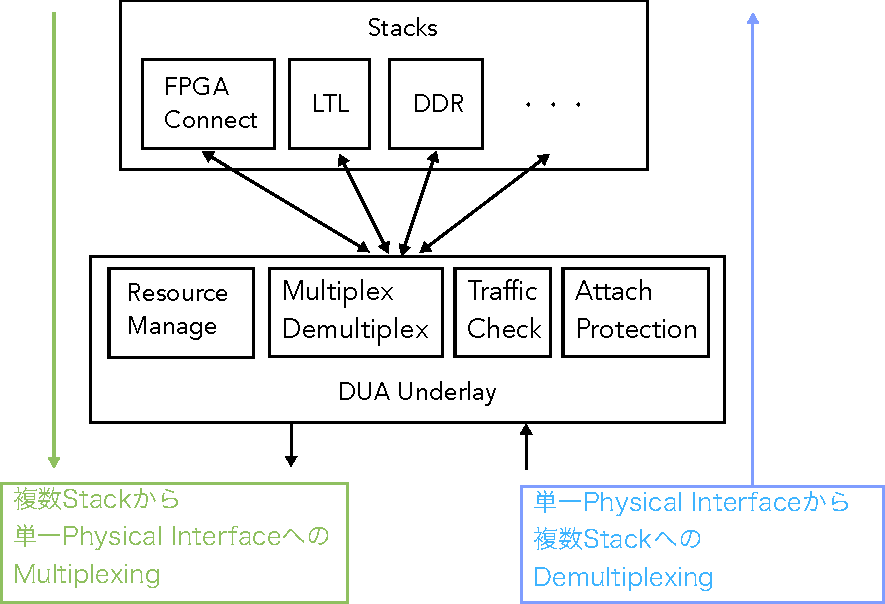
\includegraphics[scale=0.5]{fig/ez_FPGA_Underlay.pdf}
  \end{figure}
\pnote{
	次の図を見せながら説明するといい
}
\end{frame}

% これは最後のまとめかな
\begin{frame}\frametitle{DUA Overview}
  \begin{figure}[htb]
		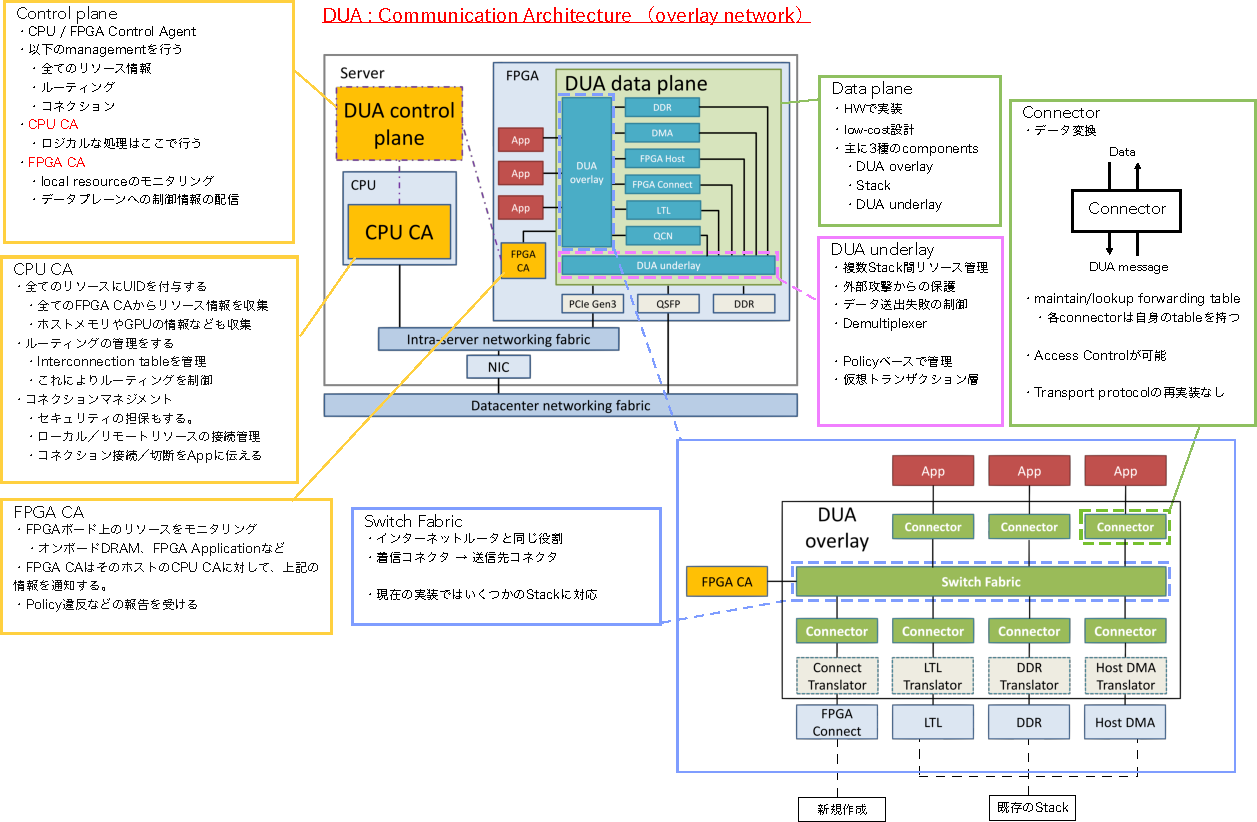
\includegraphics[width=\linewidth]{fig/ez_DUA_high_overview.pdf}
  \end{figure}
\pnote{
}
\end{frame}


% ==========================================================================

% ======================== 評価 (Microbenchmark / Application Benchmark)==============================

\section{Evaluation}
\begin{frame}\frametitle{Evaluation}
	\begin{itemize}
			\item MicroBenchmarkとApplicationBenchmarkで性能を測定
			\item Testbetとしては下図
				\begin{itemize}
					\item Server : Supermicro SYS-4028GR-TR2 x 2 (一部の検証ではDell R720) with 40Gps NIC
					\item FPGA : Altera Stratix V D5, 172.6K ALMs, 4G DDR3-1600 DRAM, PCIe Gen3 x8, 40GbE QSFP+ x2
					\item Switch : Arista 706 0X
					\item OS : Windows Server 2012 R2
				\end{itemize}
	\end{itemize}
  \begin{figure}[htb]
		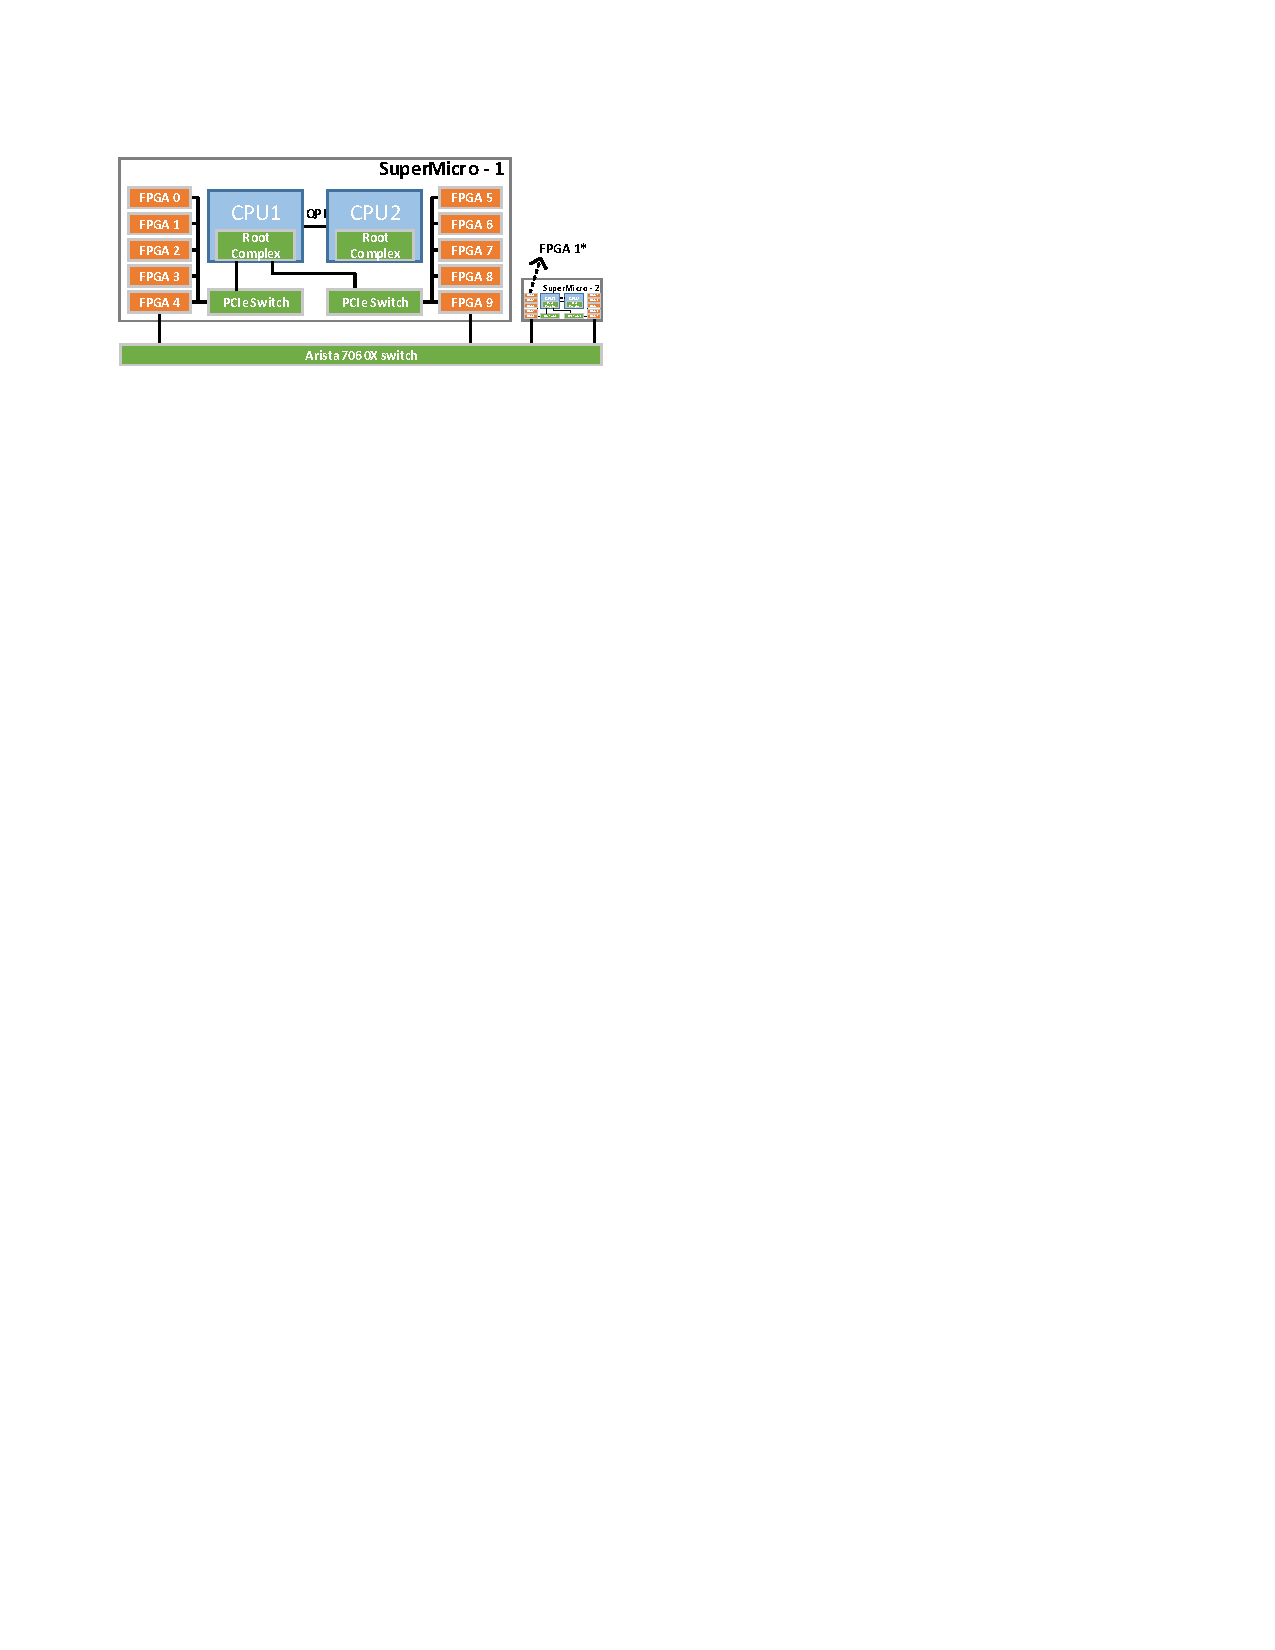
\includegraphics[scale=1.0]{fig/figure9.pdf}
  \end{figure}
\pnote{
	Altera Stratix V D5はミドルレンジFPGAと書いてあったがほんまか?
}
\end{frame}

\begin{frame}\frametitle{MicroBenchmark : FPGA Area Cost}
	\begin{itemize}
			\item DUAの実装に関わるFPGAリソースの消費の関係が下の表
			\item 4 stack (4-port switch, 4 connectors, 4 stack translator) には9.29\%
			\item Application側に4port追加しても19.86\%
			\item Underlayは4 stack - 3 physical interfaceで0.25\%
			\item Area costとしては低いし許容範囲\\(ハイエンドFPGAでは無視できるレベル)
	\end{itemize}
  \begin{figure}[htb]
		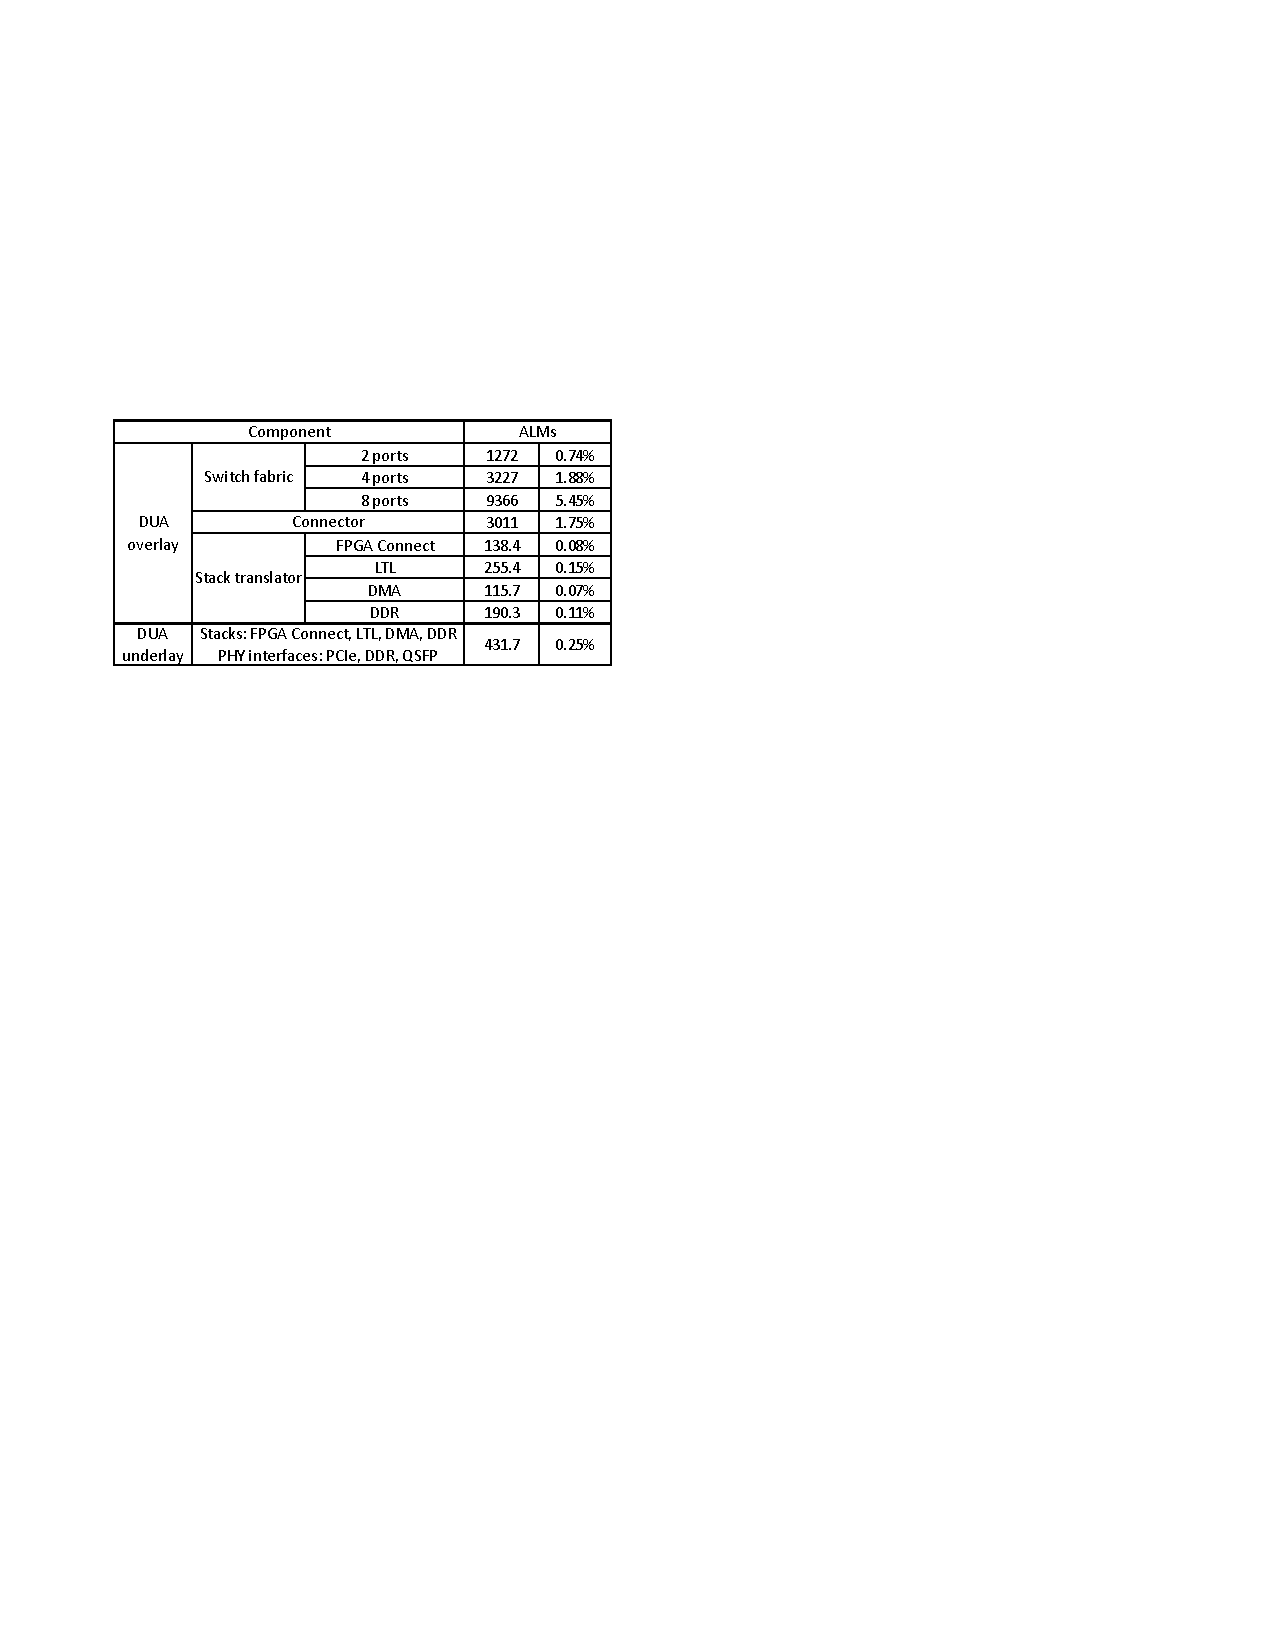
\includegraphics[scale=1.0]{fig/figure10.pdf}
  \end{figure}
\pnote{
	ハイエンドなら無視できるとあるがちょっとこの辺はわからない
}
\end{frame}

\begin{frame}\frametitle{MicroBenchmark : Switch Fabric Performance}
	\begin{itemize}
			\item スイッチファブリックの性能評価
				\begin{itemize}
    			\item 全switch portはtraffic generator/result checkerのapplicationに接続する
    			\item 混雑したトラフィックシナリオを想定してメッセージ送信
    			\item メッセージサイズは32Bから4KBまで変化
    			\item switch fabricは300MHzで動作、理想のスループットは9.6GBpsとのこと。
    			\item 2時間のテストでLatency / Throughputを計測。
				\end{itemize}
			\item スループットは理論上の最大値に到達 \& レイテンシは低い
	\end{itemize}
  \begin{figure}[htb]
		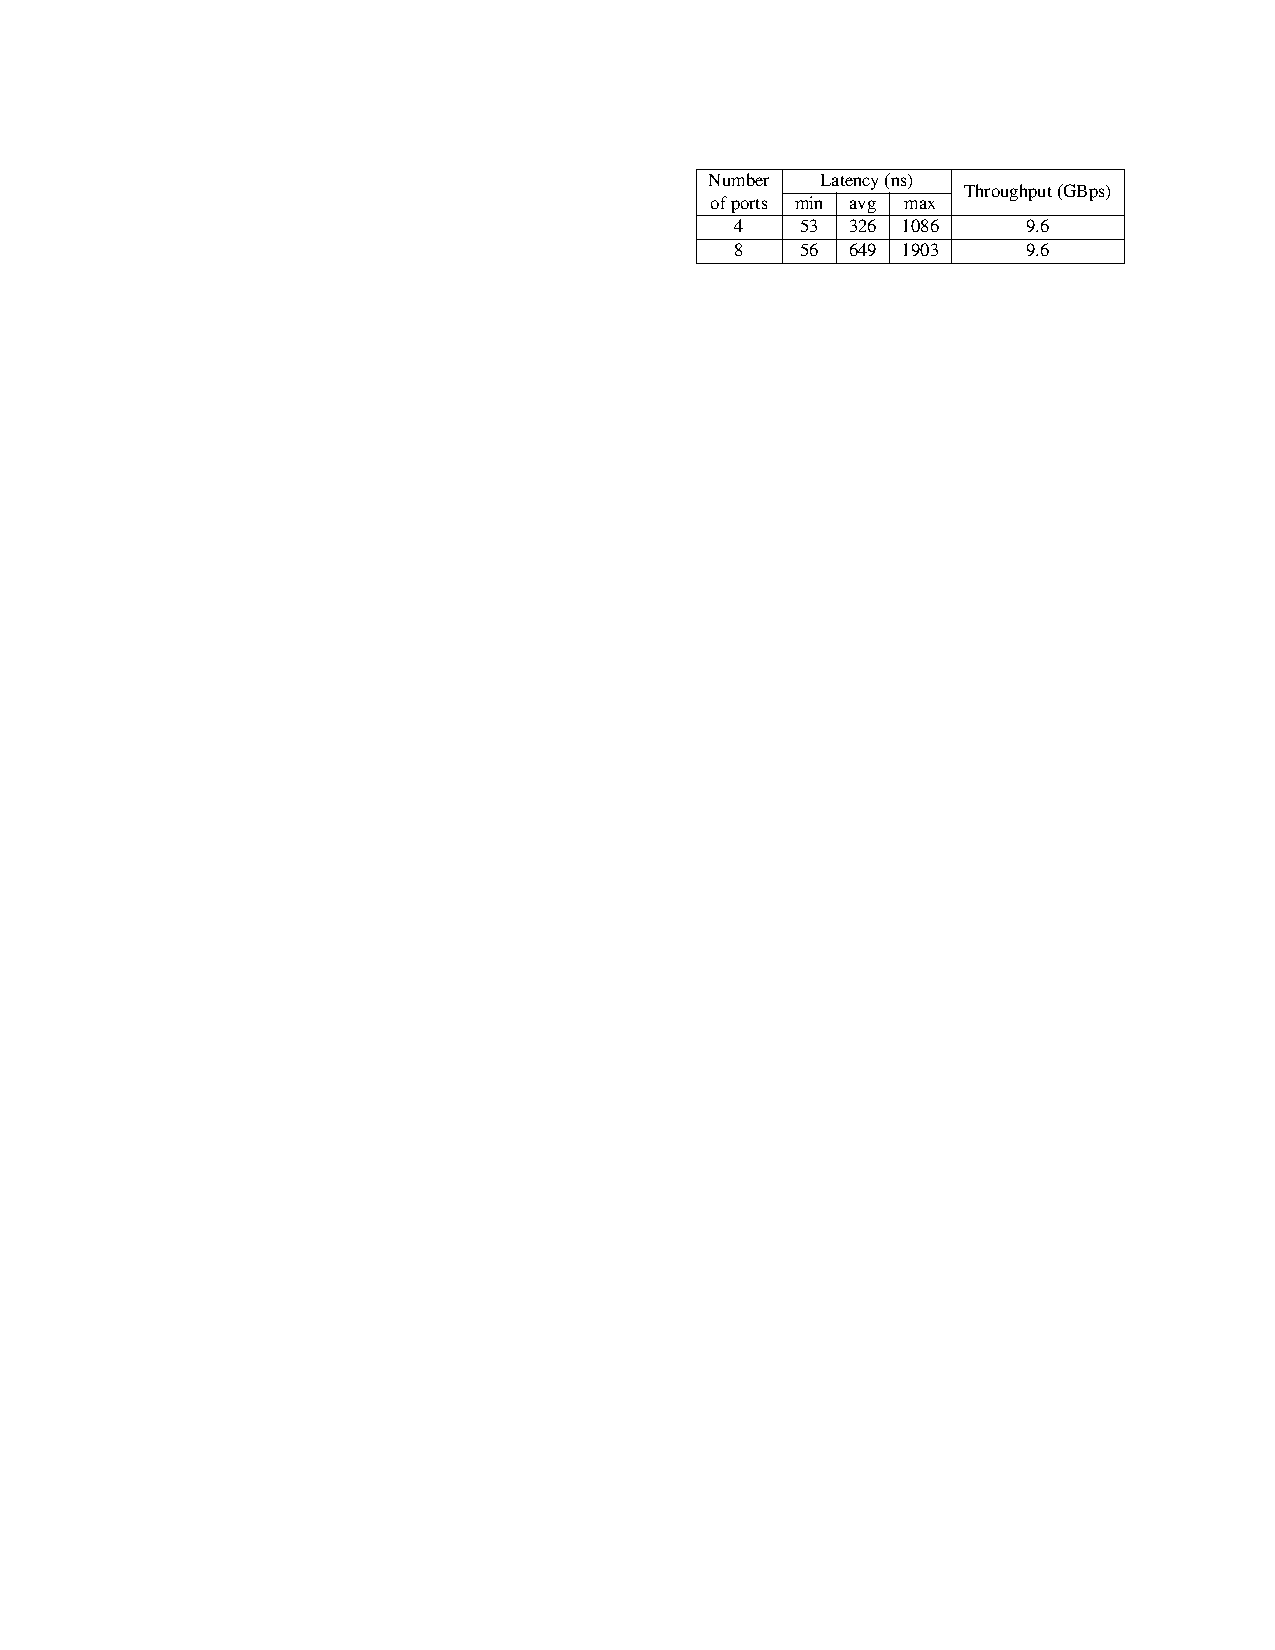
\includegraphics[scale=1.0]{fig/table2.pdf}
  \end{figure}
\pnote{
}

\end{frame}
\begin{frame}\frametitle{MicroBenchmark : Routing Table Performance}
	\begin{itemize}
			\item おそらくConnectorでのForwarding Table matchingの部分だと思う。。。
			\item 詳細がないが、Table entryに対するmatching engineを組んだとのこと。
			\item tableエントリと1portあたりのエリアコスト、及び最大周波数をまとめた結果が下
				\begin{itemize}
					\item 32エントリのとき1portあたり0.83\%エリアコスト、4-8portで考えると3.3\%-6.6\%程度
					\item エントリ数が増加するとエリアコストはリニアに増加するが、最大周波数の減少はそれほど低下しない
					\item このときのメッセージサイズの情報が書いてなかったが、message-per-secondのThroughputがclock frequencyとおなじになる実装らしく、1portあたり10GBps位出るらしいので、計算するとだいたい1message=20Byte程度と思われる(多分)
				\end{itemize}
	\end{itemize}
  \begin{figure}[htb]
		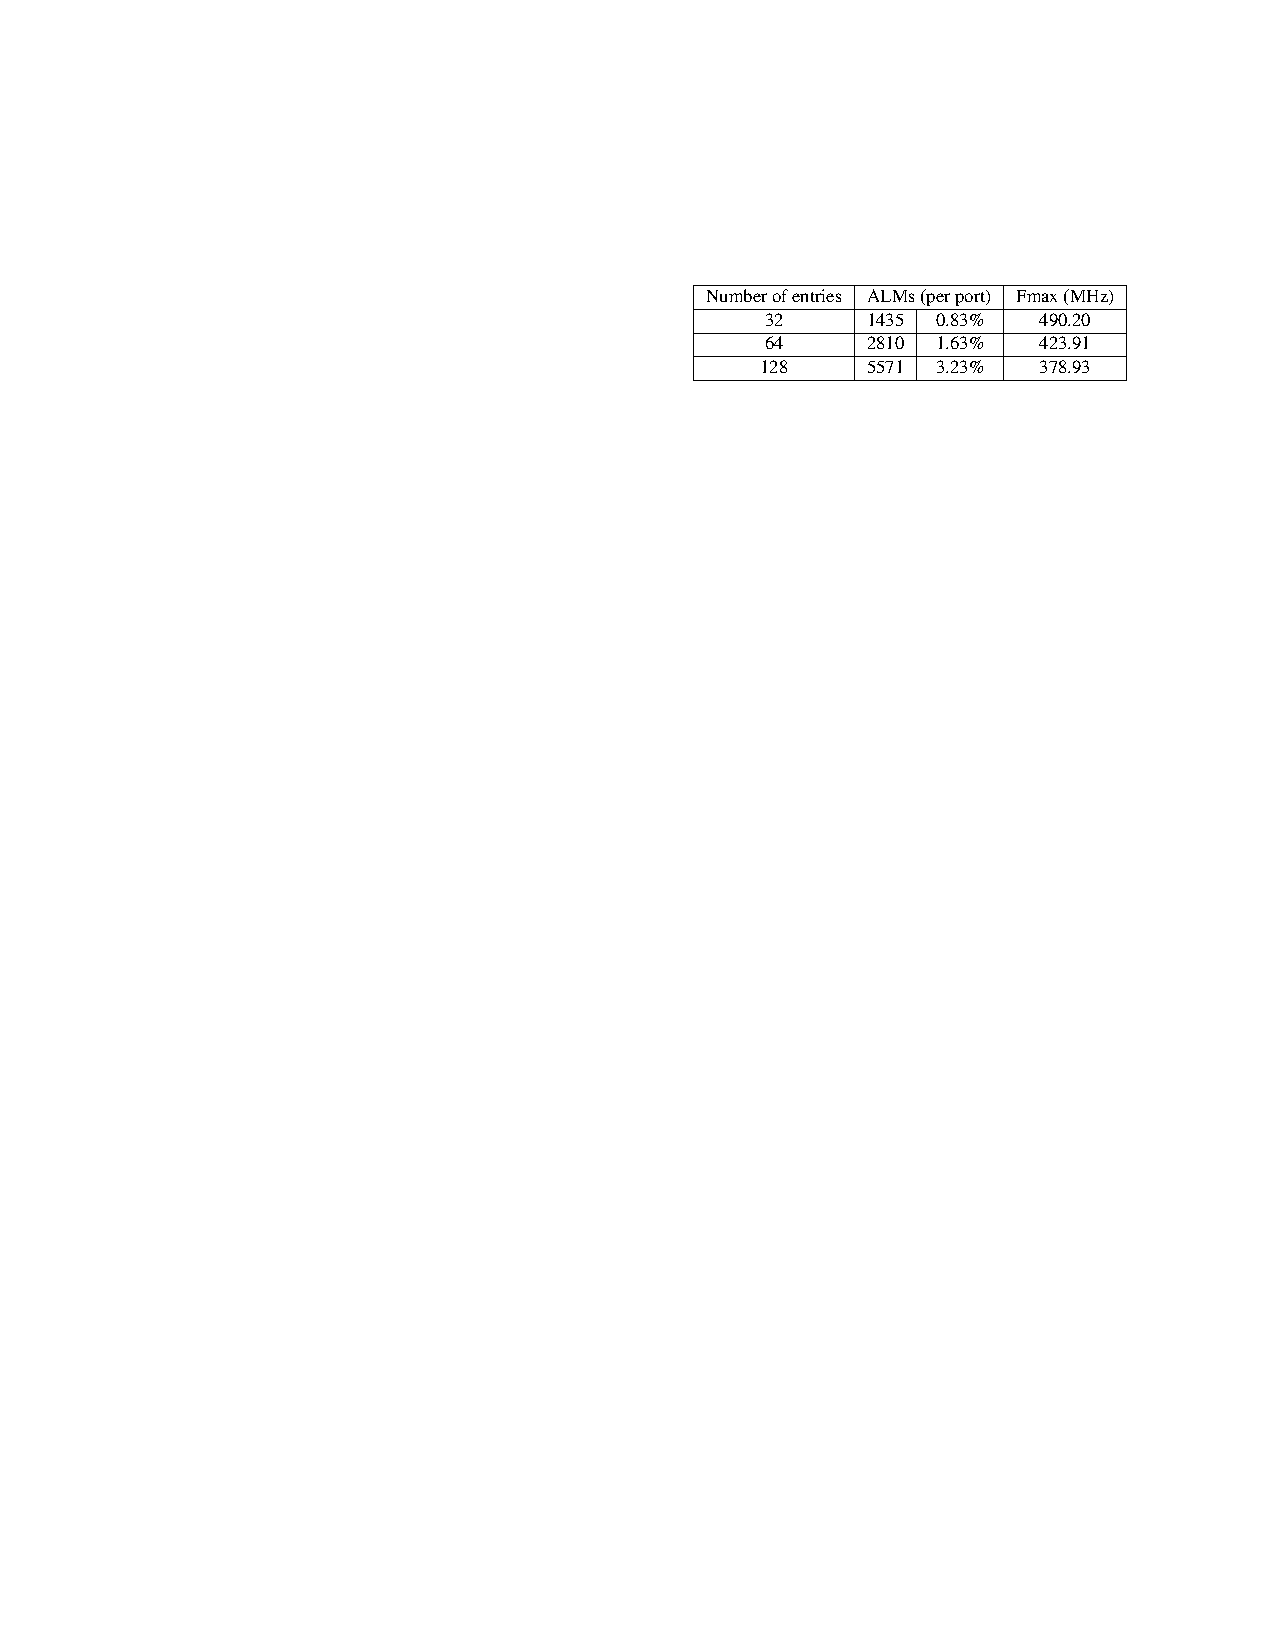
\includegraphics[scale=1.0]{fig/table3.pdf}
  \end{figure}
\pnote{
  これちょっと難しいな(最大周波数とThroughput)
  1sで490M回cycleする。
  1sで490Mmessageのmatchingを行う
  1message = x Byte
  Throughput (Byte/s) = 490M * x
  (逆に) 10000 (MBps (10GBps)) / 490(MBps) = x = 20.4くらい
  messageサイズの情報がなかった
}
\end{frame}

\begin{frame}\frametitle{Microbenchmark : Latency Overhead}
	\begin{itemize}
		\item FPGA1からFPGA1$^{*}$へのデータ送信
			\begin{itemize}
				\item[1] FPGA1 $\rightarrow$ FPGA4へFPGA Connect でデータ送信
				\item[2] FPGA4 $\rightarrow$ FPGA4$^{*}$へLTLでデータ送信
				\item[3] FPGA4$^{*}$ $\rightarrow$ FPGA1$^{*}$へFPGA Connectでデータ送信
			\end{itemize}
		\item end-to-endの通信レイテンシを各レイテンシごとに確認
		\item Stackレイテンシに比べ、DUAのレイテンシ無視できるくらいはかなり低い
	\end{itemize}
  \begin{figure}[htb]
		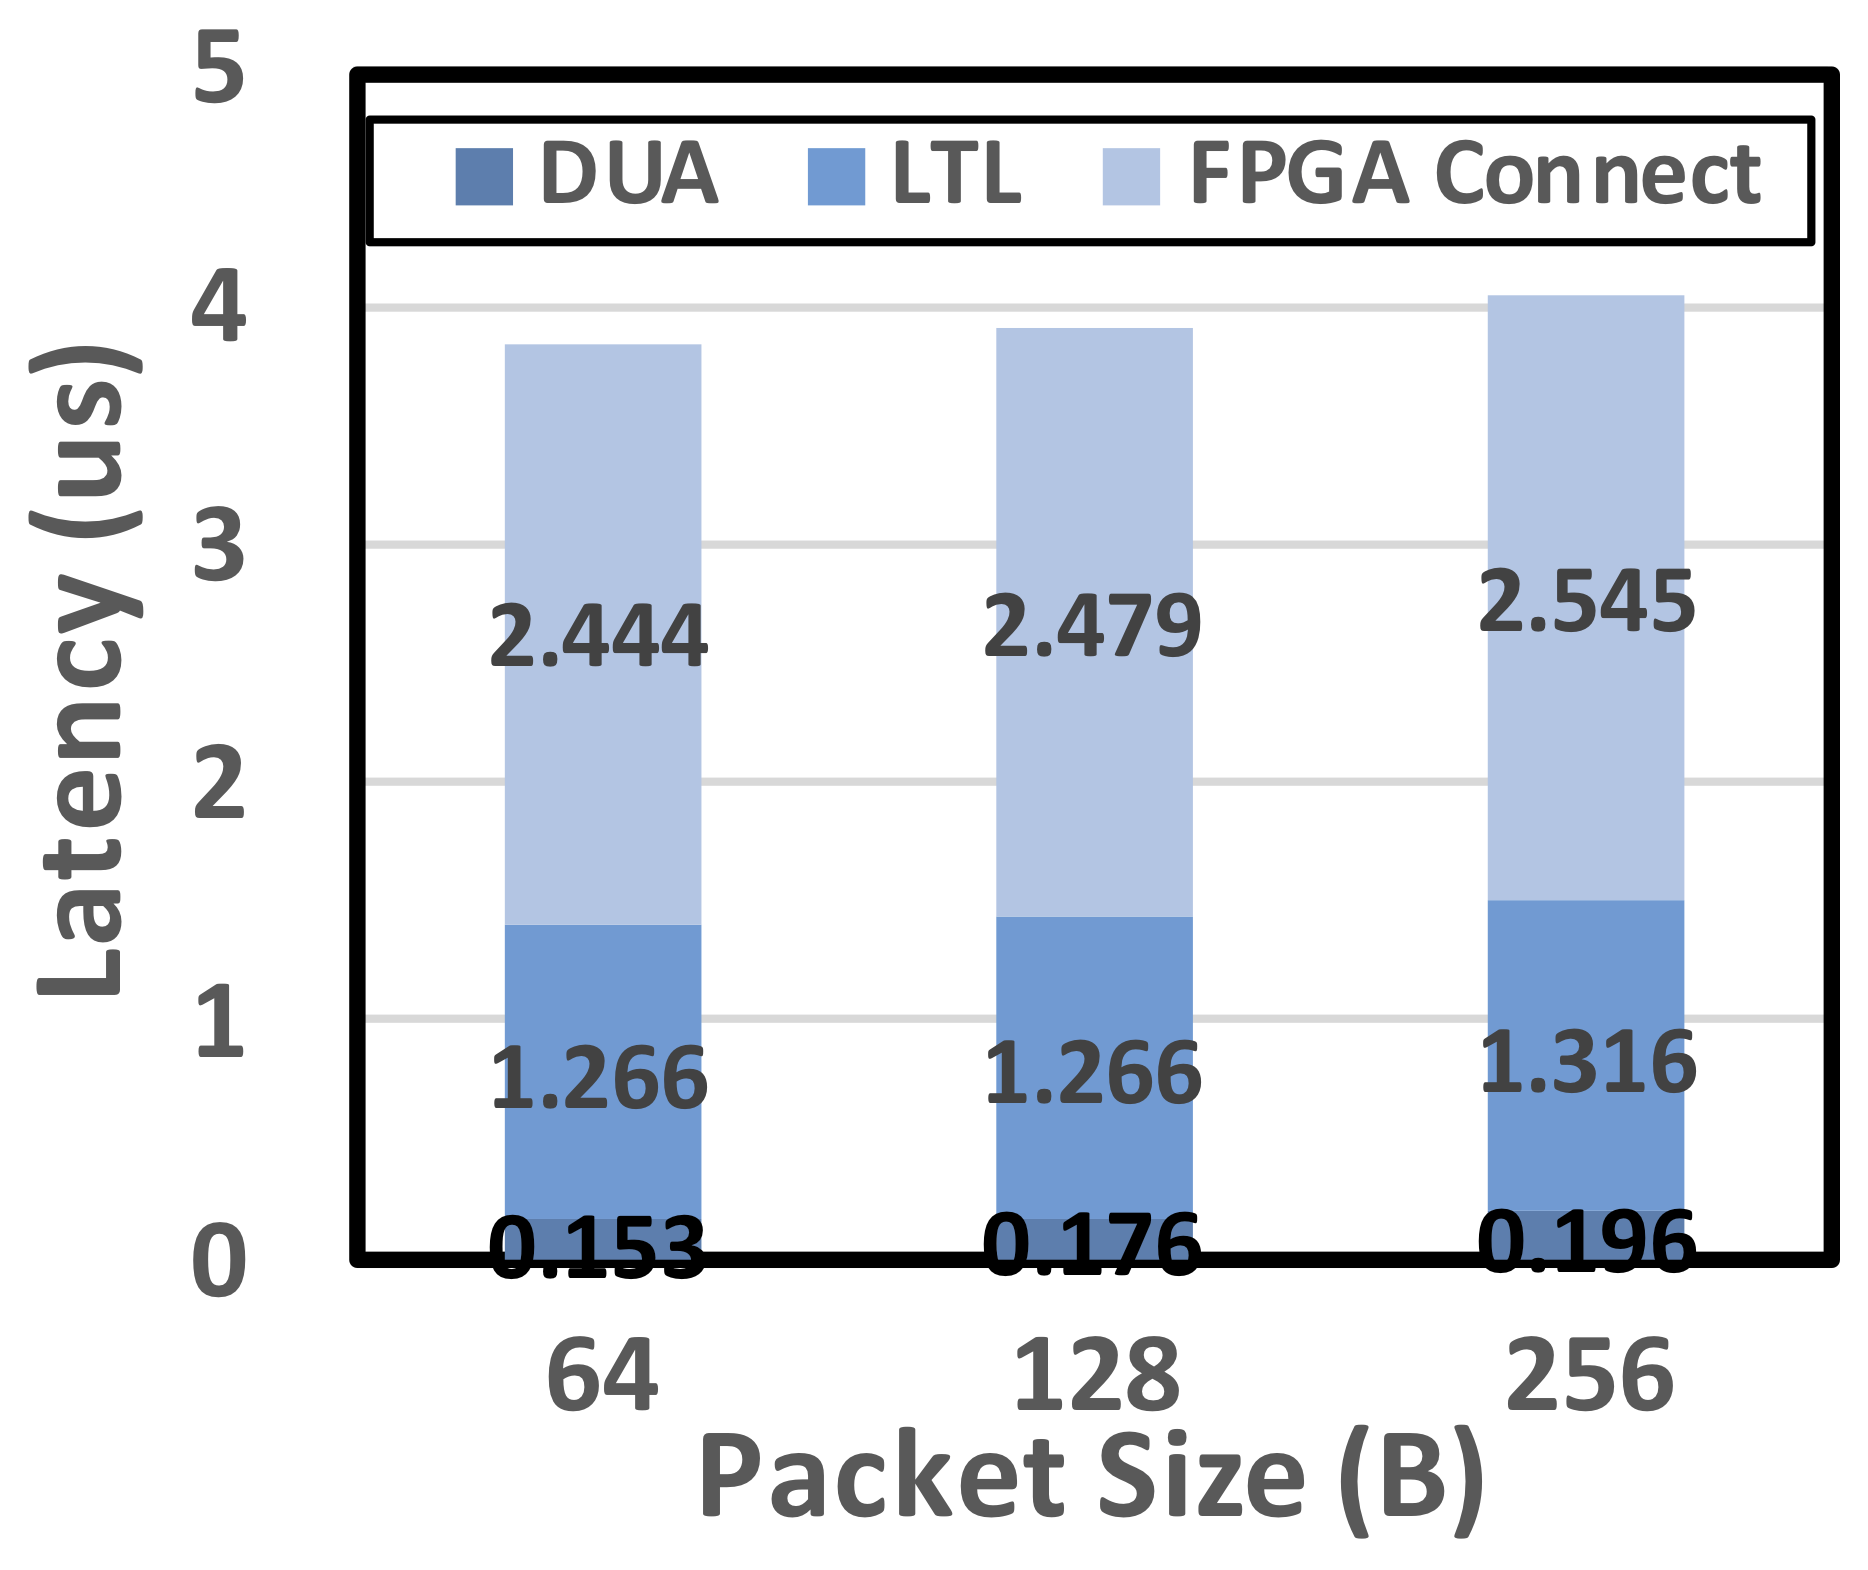
\includegraphics[scale=1.0]{fig/figure11a.png}
  \end{figure}
\pnote{
}
\end{frame}

\begin{frame}\frametitle{MicroBenchmark : Handling Multiplexing}
	\begin{itemize}
			\item DUAのMultiplexing性能の測定
				\begin{itemize}
					\item 同一のPCIe interfaceでHost DRAMにデータを書き込むApplication1, 2, 3で重みを途中で変えて(weight 1:1:2)を時間をずらしながら実行
					\item 0sでApp 1を実行
					\item 1sでApp 2を実行すると、App 1と合計してTotal Throughputに達成するように平等にスケジュールされる
					\item 2sでApp 3を実行すると、これも平等にスケジュリング
					\item 3sで重みを反映すると、重みに従った分布になる
				\end{itemize}
			\item 期待されるThroughputへの切り替わりもかなり早い
	\end{itemize}
  \begin{figure}[htb]
		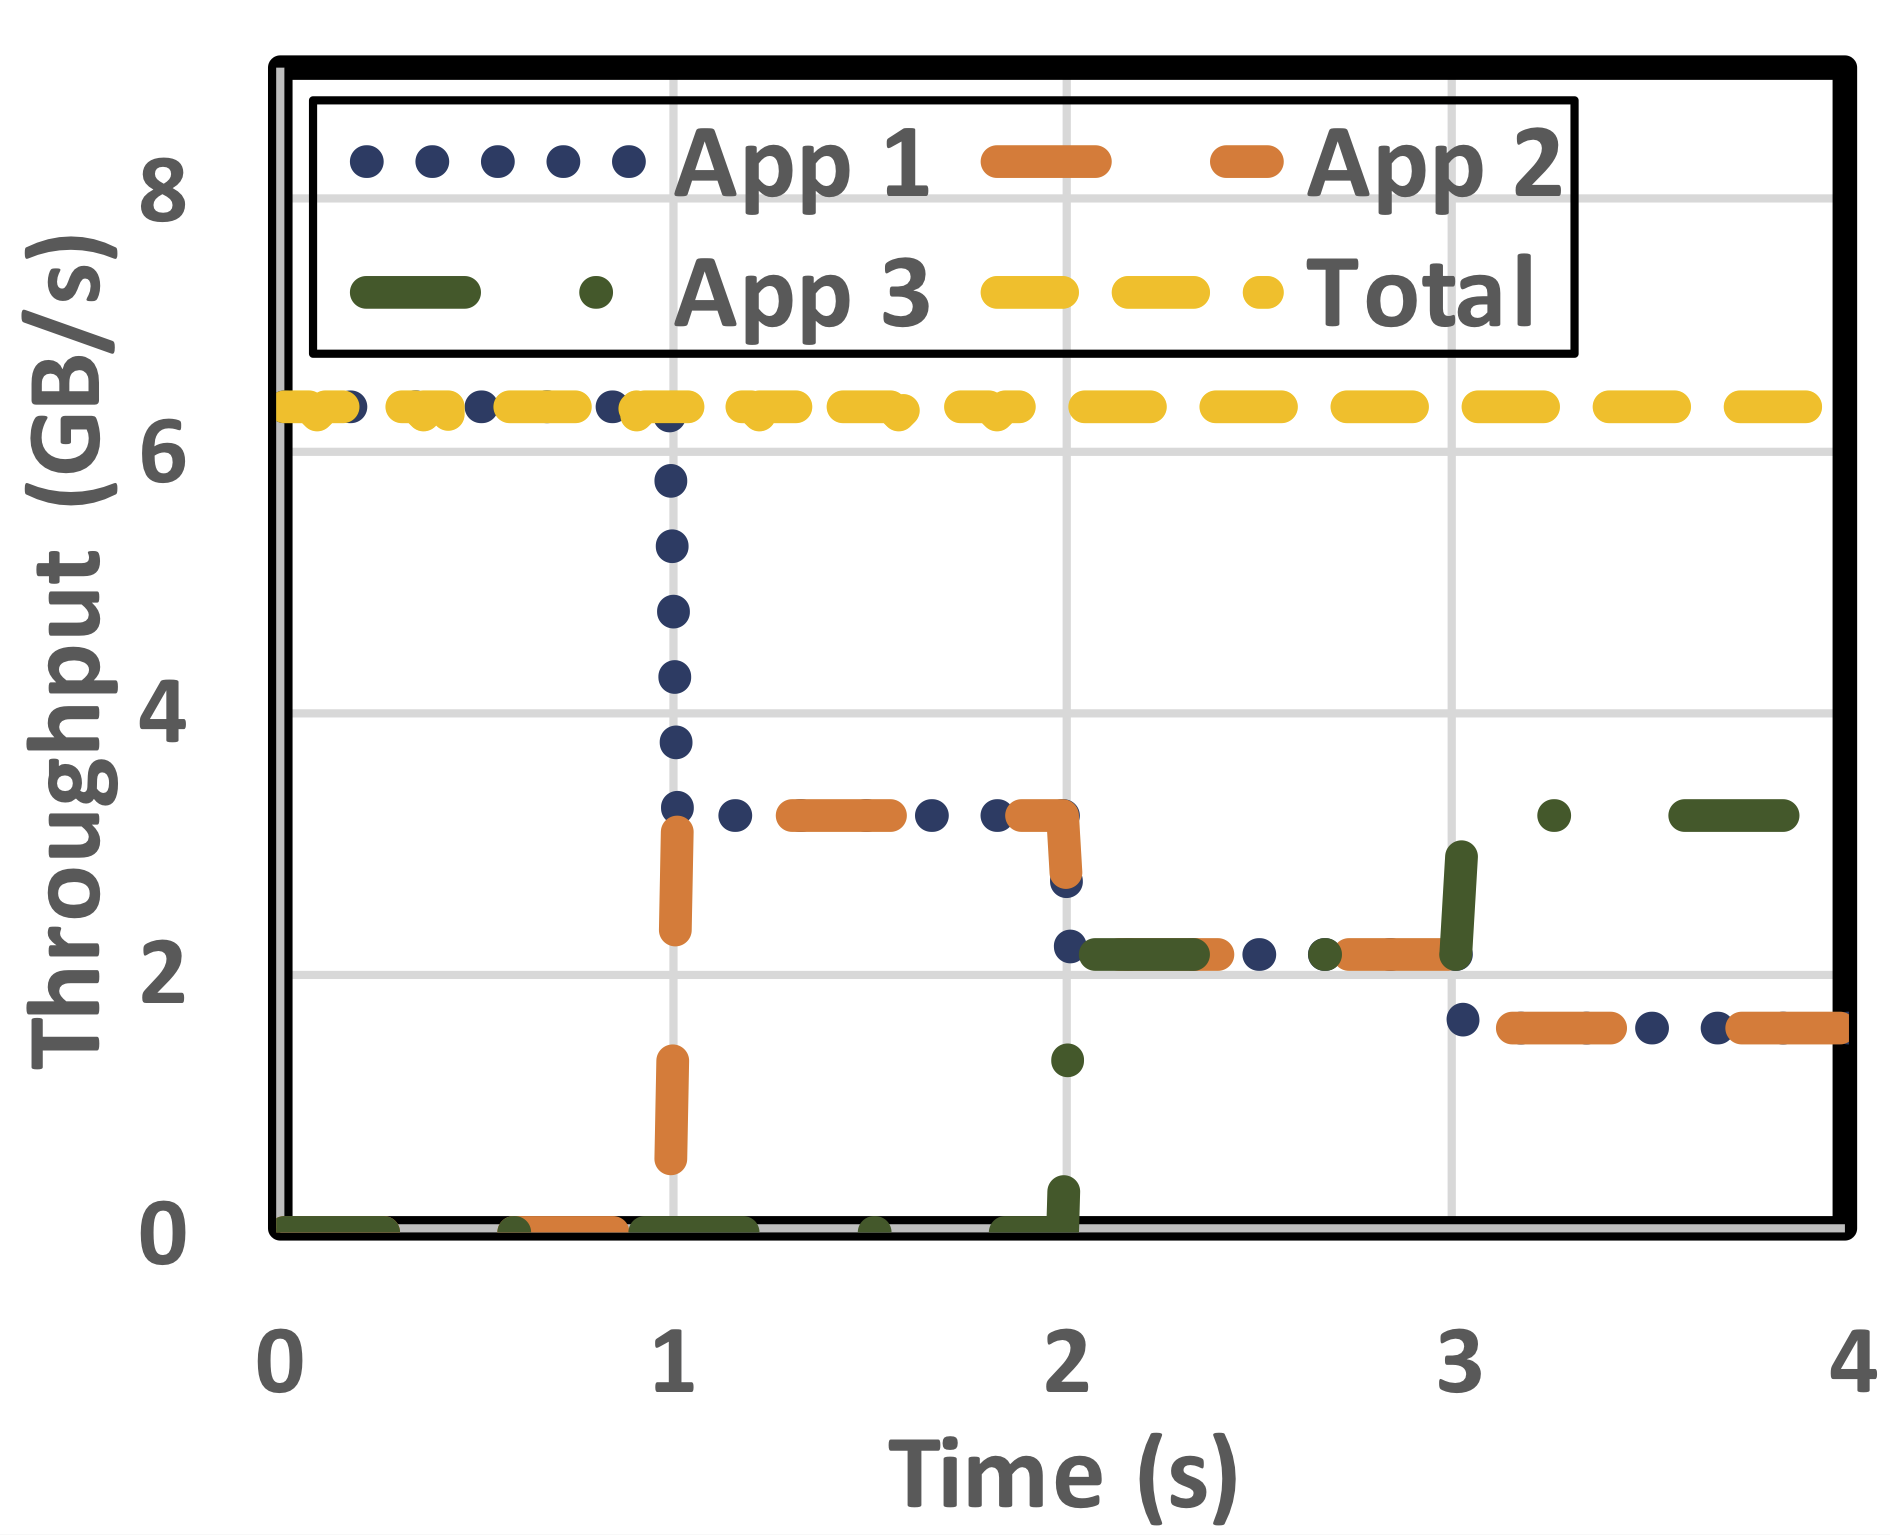
\includegraphics[scale=1.0]{fig/figure11b.png}
  \end{figure}
\pnote{
}
\end{frame}

% 今回の彼らの実装では並列度をパラメータ化している
\begin{frame}\frametitle{ApplicationBenchmark : Deep Crossing}
	\begin{itemize}
			\item Bingで使用されているらしいdeep neural networkらしい
			\item サービス応答に関わるレイテンシが重要
			\item モデル構造のうちの一部がベクトル計算集約的な部分のためそれをFPGAにoffloadし処理時間を短縮する
			\item 並列度をパラメータ化すると処理完了時間が短縮できるがロジックリソース消費量が増える
			\item 今回モデル内DVM全てを並列度64で実装し、最初2つと後ろ2つを分けてFPGAx2で実装する
			\item 接続方式はFPGA Connect / LTL で確認
	\end{itemize}
  \begin{figure}[htb]
		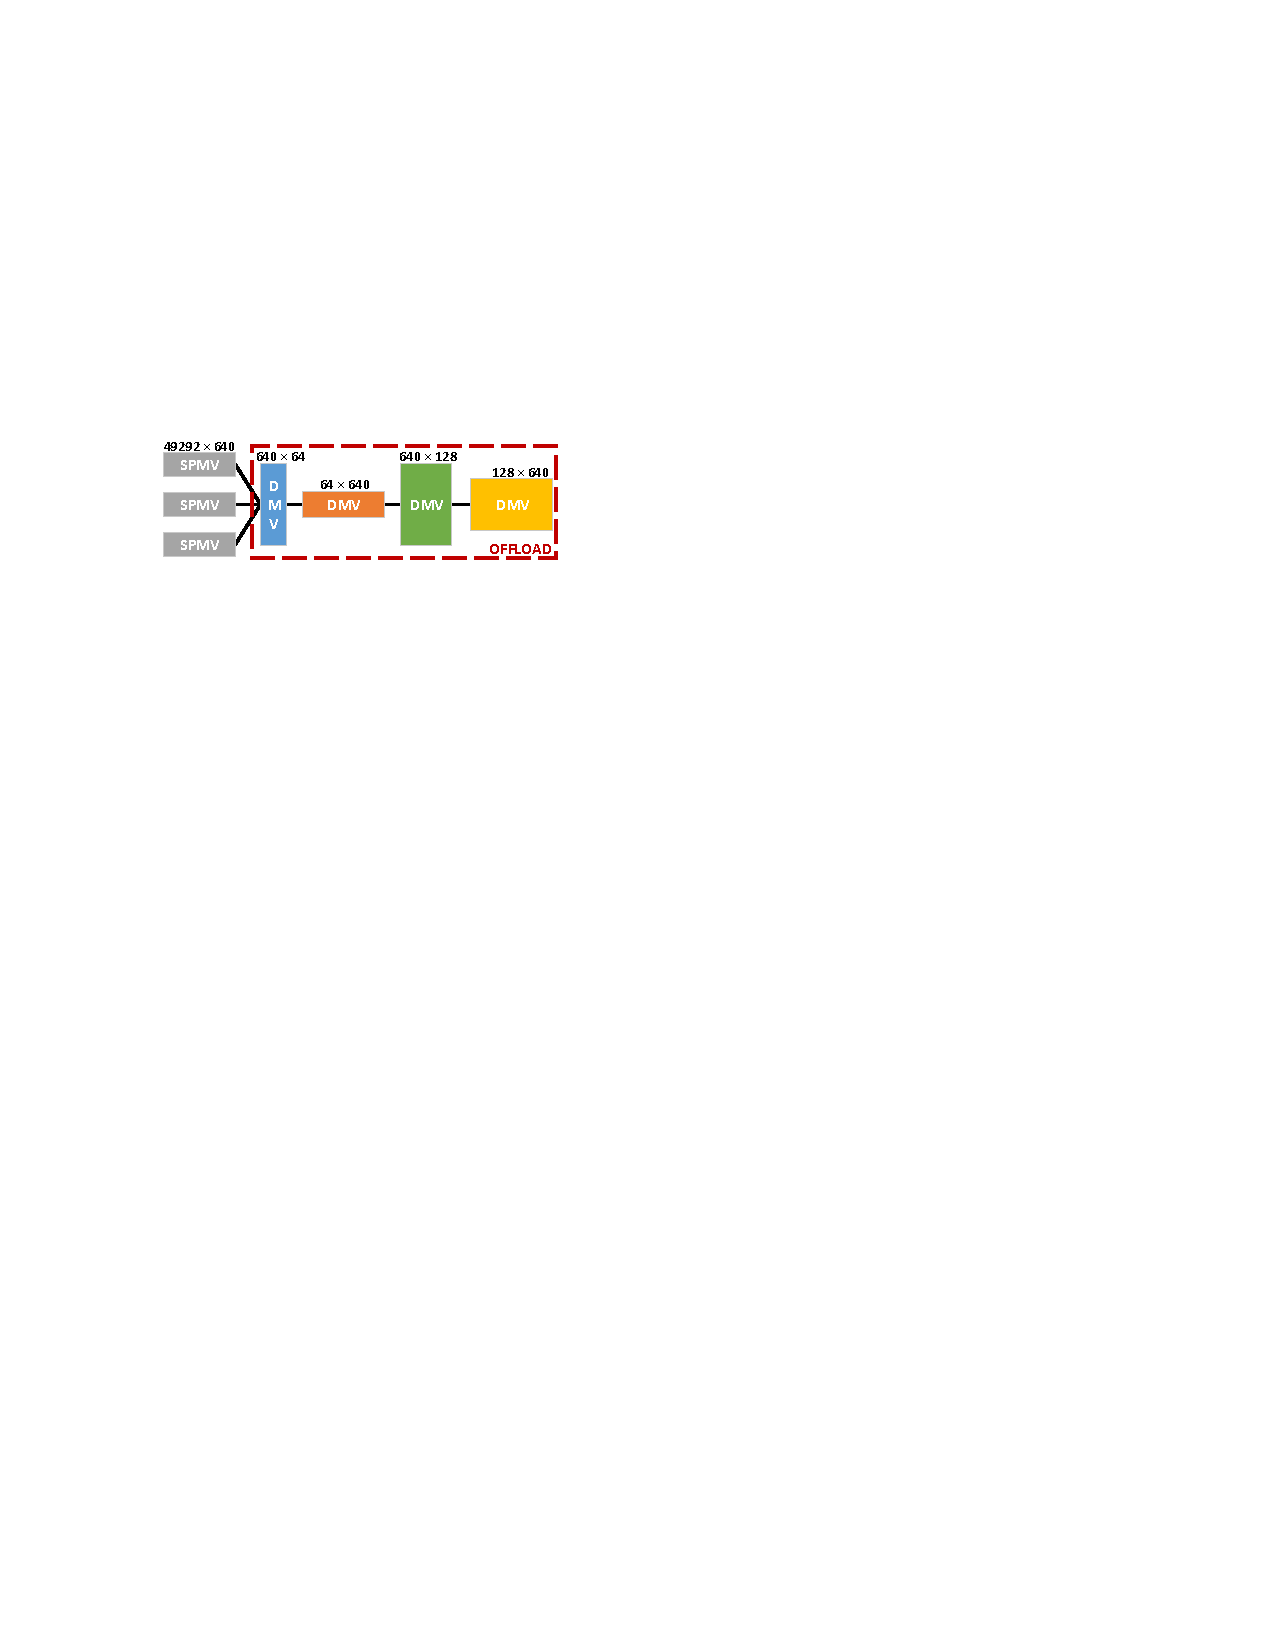
\includegraphics[scale=1.0]{fig/figure12.pdf}
  \end{figure}
\pnote{
}
\end{frame}

\begin{frame}\frametitle{Application Benchmark : Deep Crossing}
	\begin{itemize}
			\item シングルFPGAはArea Cost的に並列度32でしか実装できない。それとの比較
			\item シングルFPGAでは発生しないCommunication Latencyが発生している
			\item 一方DVMごとの並列度が上がっているので、処理時間は向上しレイテンシはFPGA Connectでは約42\%、LTLでは約37\%削減
			\item 2つのFPGAボードを繋ぐために必要な追加のOpenCLコード数は26行だった
	\end{itemize}
  \begin{figure}[htb]
		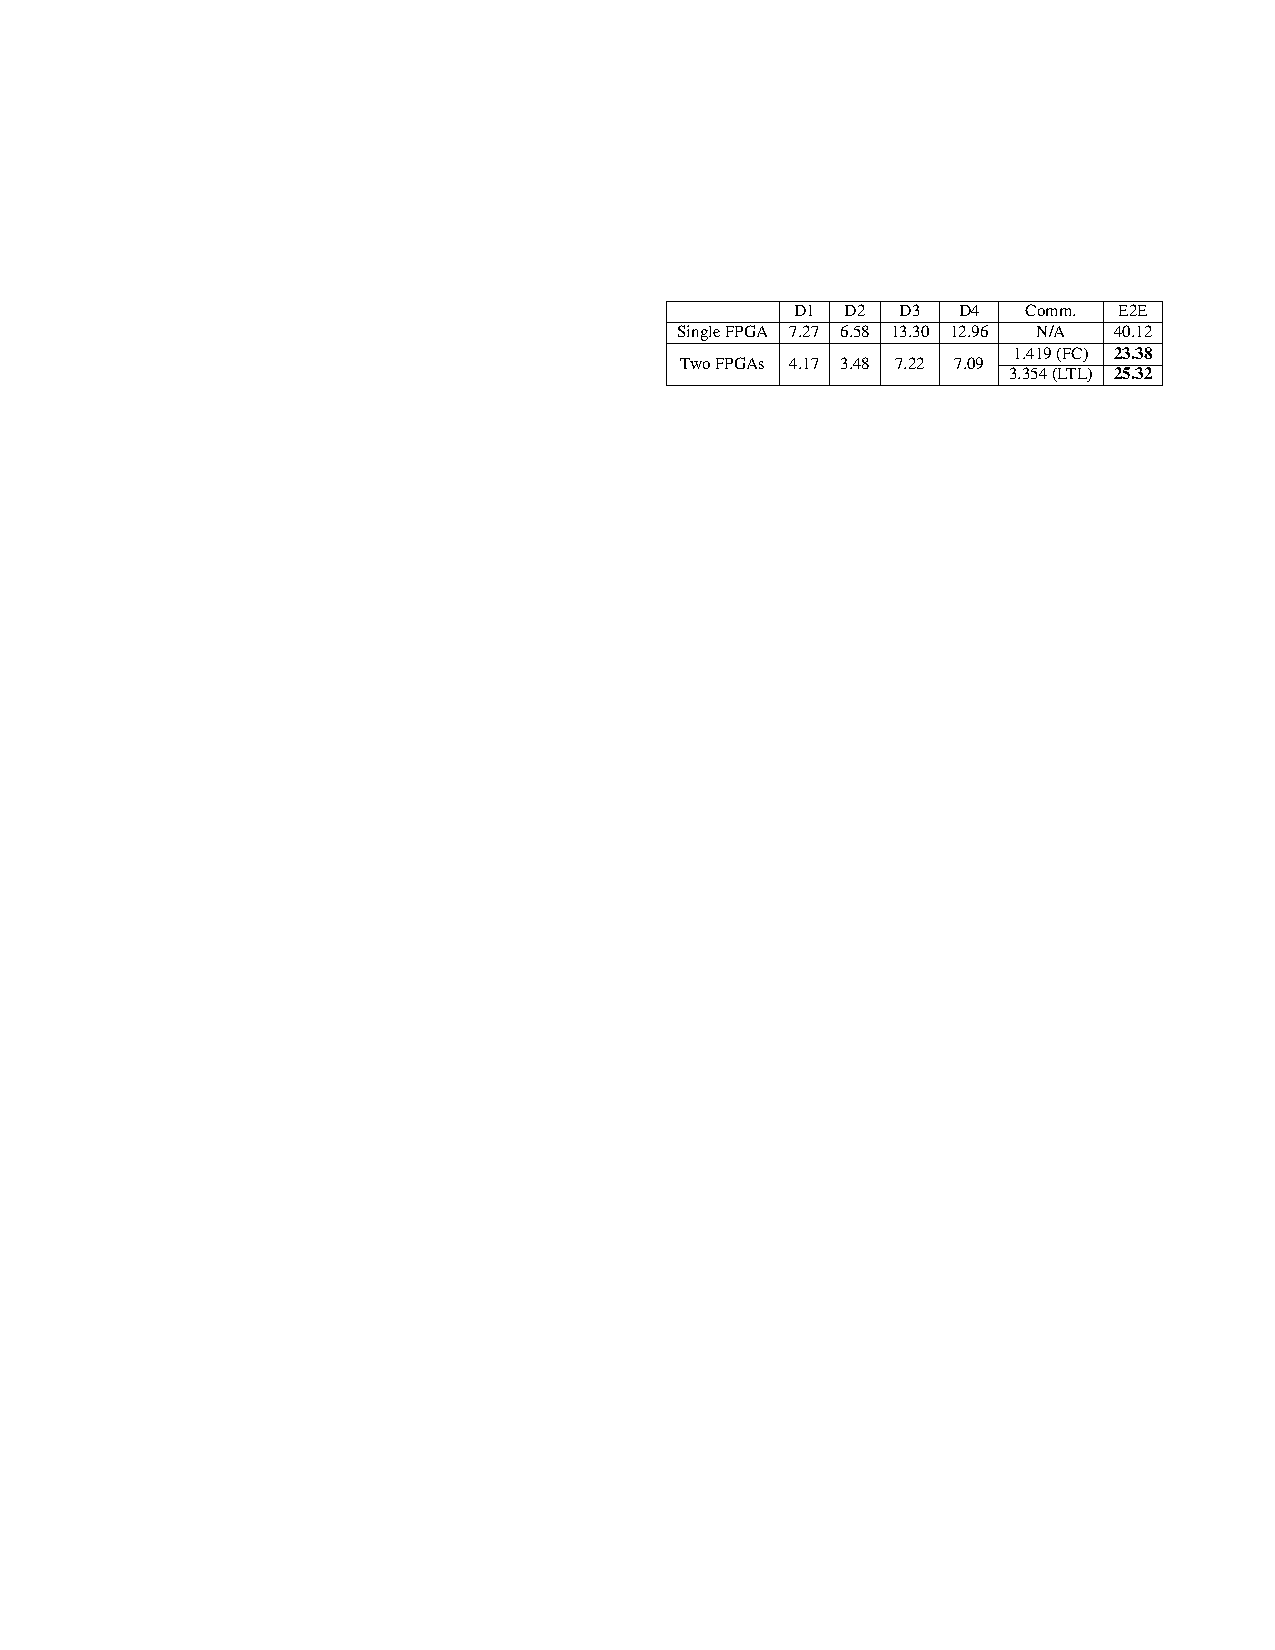
\includegraphics[scale=1.0]{fig/table5.pdf}
  \end{figure}
\pnote{
	前のLatencyのデータと比べて、データおかしくない
}
\end{frame}

\begin{frame}\frametitle{ApplicatonBenchmark : Multi-Regular-Expression Matching}
	\begin{itemize}
		\item IDS(侵入検知システム)では典型的に正規表現が利用されるそうな
    \item DUA上の3FPGAで構成されるfast multi-regular-expression matching プロトタイプを作成し測定
		\item 219の正規表現ルールを作成し、3分割(73rules/stg)してステージ分けし、それぞれのステージを各FPGAで実装した。
		\item 並列度は32, 1cycleで8bit文字列をマッチングし、入力文字列がステージで照合完了して初めて次のステージに送られる
		\item 接続方式はFPGA Connect, 比較対象はCPUを通じたFPGA間のデータ転送時、及びCPUでのマッチング性能。
	\end{itemize}
\pnote{
}
\end{frame}

\begin{frame}\frametitle{ApplicatonBenchmark : Multi-Regular-Expression Matching}
	\begin{itemize}
		\item LatencyとThroughputを測定
		\item Throughput : 文字列が大きくなると顕著になり、CPUを通じたデータ転送と比較しても2倍程度出る
		\item Latency : CPUを通じたデータ転送と比較してもあまり変化がないが、CPU処理と比べると3倍近く高速になっていることがわかる
		\item 3つのFPGAをつなぐために必要な追加のOpenCLコード数は30行未満だった
	\end{itemize}
  \begin{figure}[htb]
		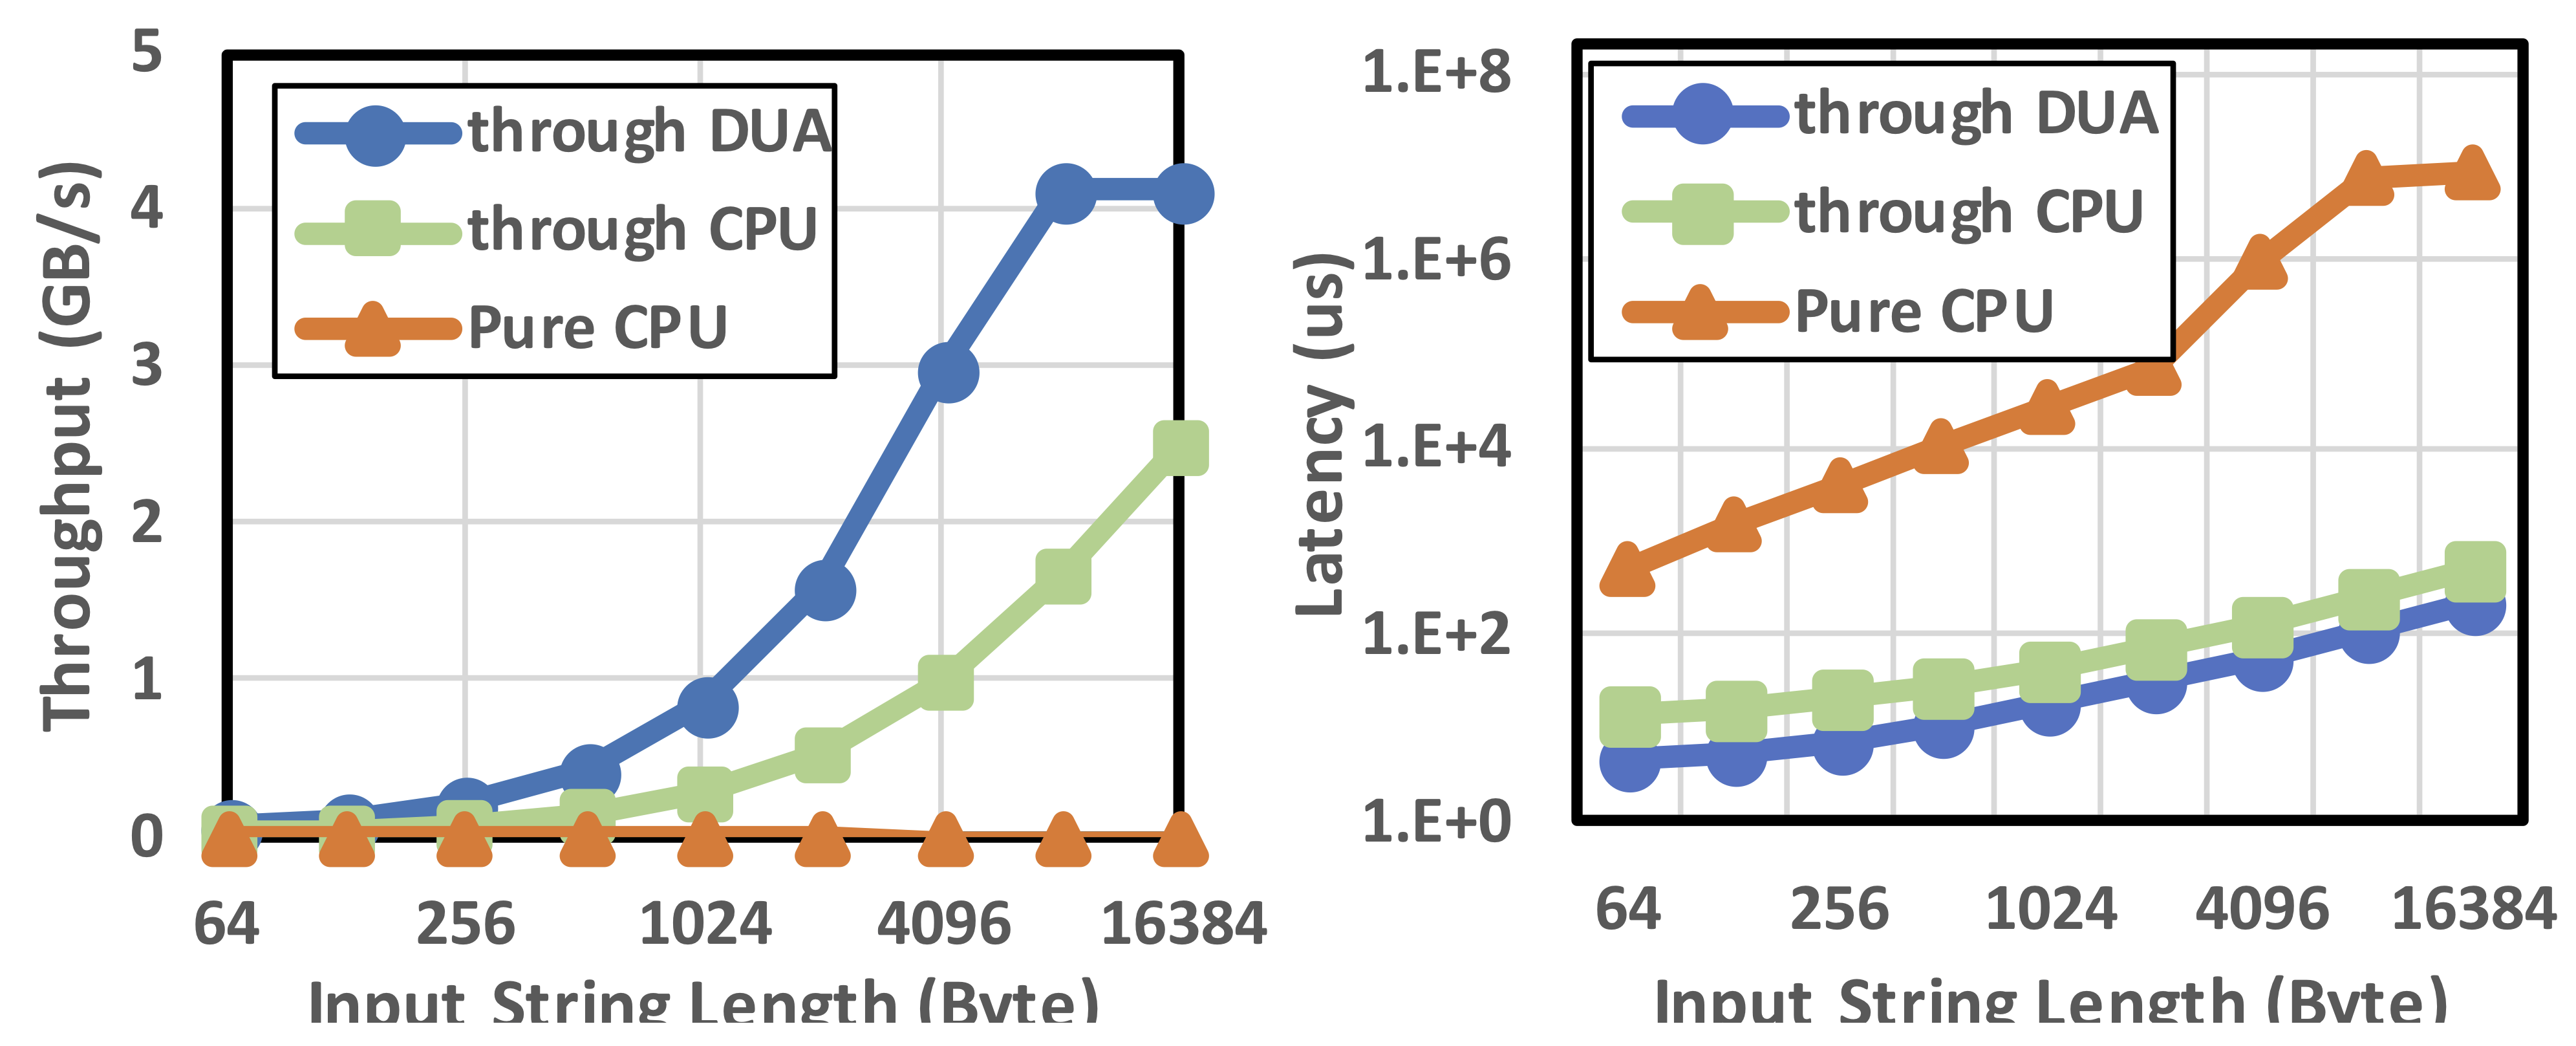
\includegraphics[scale=1.0]{fig/figure13.png}
  \end{figure}
\pnote{
	比較対象に注意
	through CPUは処理自体をFPGAでやるがデータ転送部分をFPGA ConnectではなくCPUを通じてFPGA間のデータ転送をしている。
	そのため、Throughputという点ではデータ転送帯域の差が如実に出ているように見える。input文字列長がながければ長いほどその結果が顕著に出てる感じ
	対してレイテンシの観点からでは差があまりない。トータルレイテンシのうちに占めるFPGAの処理時間が大きいのかなと思います。またもちろんFPGA Connectのほうが早いけど結局同一サーバー内だし、最大でも16KB程度なので転送速度の差がグラフ上で明確に出るほどではないのかなと思った。
}
\end{frame}

\section{結論}
\begin{frame}\frametitle{Conclusion}
	\begin{itemize}
		\item FPGAのDC利用を考えたときに出てくる各種問題を解決するような理想的なアーキテクチャを考え実装した
		\item FPGAからDCネットワークのリソースを容易に利用できるようになった。
		\item 実装に関わるArea Costも低く、性能もLatency/Throughputの観点から非常に良いことがわかった。
	\end{itemize}
\pnote{
}
\end{frame}


\newcounter{finalframe}
\setcounter{finalframe}{\value{framenumber}}
\setcounter{framenumber}{\value{finalframe}}
\end{document}
